%% %%% NT includes
%% \documentclass{ntmanuscript}
%% \bibliographystyle{ans}
%% \usepackage{cite} % for ans
%% %%%

%%% ELS includes
\documentclass[review]{elsarticle}
\usepackage{lineno,hyperref}
\modulolinenumbers[5]
\journal{Nuclear Engineering and Design}
\bibliographystyle{elsarticle-num}
%%%

%%% General usepackages, definitions, etc.

%%%%% Packages and related options
%%
%% Note, order matters!
%%
\usepackage[acronym,toc]{glossaries}
\usepackage{graphicx}
\usepackage{booktabs} % nice rules for tables
\usepackage{microtype} % if using PDF
\usepackage{hyperref}
\usepackage{amsmath}
\usepackage{moreverb} % for verbatim snippets of code
\usepackage{fancyvrb}
\usepackage{tabularx} % for tables with line breaks
\usepackage{threeparttable} % for tables with notes
\usepackage[capitalize, noabbrev]{cleveref} % for reference multiple figures
\usepackage{calc} % allows for arithmetic on latex variables
\usepackage{float} % allows for figures to be placed explicitly
\usepackage{algorithm2e} % for algorithms
\usepackage{subfig}
\usepackage{multirow} % combining rows in tables
\usepackage{footnote}
\usepackage{titlesec} % for using \titleformat
\usepackage{slashbox} % for tables with a divided cell, see http://tex.stackexchange.com/questions/7262/diagonally-divided-table-cell
\usepackage{bashful}
\usepackage{xspace}
\usepackage{color}
\definecolor{listinggray}{gray}{0.9}
\definecolor{lbcolor}{rgb}{0.9,0.9,0.9}
\lstset{
    %backgroundcolor=\color{lbcolor},
    language={C++},
    tabsize=4,
    rulecolor=\color{black},
    upquote=true,
    aboveskip={1.5\baselineskip},
    belowskip={1.5\baselineskip},
    columns=fixed,
    extendedchars=true,
    breaklines=true,
    prebreak=\raisebox{0ex}[0ex][0ex]{\ensuremath{\hookleftarrow}},
    frame=single,
    showtabs=false,
    showspaces=false,
    showstringspaces=false,
    basicstyle=\scriptsize\ttfamily\color{black},
    keywordstyle=\color[rgb]{0,0,1.0},
    commentstyle=\color[rgb]{0.133,0.545,0.133},
    stringstyle=\color[rgb]{0.627,0.126,0.941},
    numberstyle=\color[rgb]{0,1,0},
    identifierstyle=\color{black},
    captionpos=t,
}
\lstdefinestyle{BashOutputStyle}{
  basicstyle=\small\ttfamily,
  numbers=none,
  frame=tblr,
  columns=fullflexible,
  backgroundcolor=\color{blue!10},
  linewidth=0.9\linewidth,
  xleftmargin=0.1\linewidth
}
%%%%% 

%%%%% Helpers

\newcommand{\Cycamore}{\textsc{Cycamore} }
\newcommand{\cyclus}{\textsc{Cyclus}\xspace}
\newcommand{\Cyclus}{\textsc{Cyclus} }
\newcommand{\nucl}[2]{\ensuremath{^{#1}}\mbox{#2}}
\newcommand{\code}[1]{\lstinline[basicstyle=\ttfamily\color{black}]|#1|}
\newcommand{\codeb}[1]{\texttt{#1}}
\newcommand{\units}[1] {\:\text{#1}}%
% scenarios
\newcommand{\basecase}{\texttt{base-case}\xspace}
\newcommand{\outage}{\texttt{outage}\xspace}
\newcommand{\tariff}{\texttt{tariff}\xspace}
\newcommand{\external}{\texttt{external}\xspace}
% facilities
\newcommand{\fabrication}{\texttt{Fabrication}\xspace}
\newcommand{\separations}{\texttt{Separations}\xspace}
\newcommand{\reactor}{\texttt{Reactor}\xspace}
\newcommand{\reactors}{\texttt{Reactor}s\xspace}
\newcommand{\storage}{\texttt{Storage}\xspace}

%%% detect beginning of sentences and capitalize appropriately
\sfcode`\.=1001
\sfcode`\?=1001
\sfcode`\!=1001
\sfcode`\:=1001
\newcommand\secref[1]{\ifnum\spacefactor=1001 Section \ref{#1}\else section \ref{#1}\fi}
% this seems like a limitation of sfcode (an error occurs if at the beginnig of
% a paragraph) Accordingly, this can be used manually as
% needed. http://comments.gmane.org/gmane.comp.tex.texhax/17631
\newcommand\Secref[1]{ Section \ref{#1}}
%%%


%%% General setup
\graphicspath{{./figs/}}
%\include{acros}
\makeglossaries

%% %%% NT input
%% 
%%%%%%%%%%%%%%%%%%%%%%%%%%%%%%%%%%%
\date{}
\title{A Novel Methodology for Determining the Dynamic Exchange of Resources in
  Nuclear Fuel Cycle Simulation}

% Authors. Separated by commas
\author{
  Matthew J. Gidden$^1$,\\
  Paul P.H. Wilson$^1$
  }

% Institutes of the authors
\institute{$^1$University of Wisconsin - Madison, Department of Nuclear Engineering and 
Engineering Physics, Madison, WI 53706}

% Information concerning the person submitting the manuscript
\submitter{Matthew Gidden}
\submitteraddress{1500 Engineering Drive, Madison, WI, USA}
\submitteremail{matthew.gidden@gmail.com}

% No more than three keywords, though each can be a phrase
\keywords{fuel cycle, simulation, optimization}
 % for nuclear tech 
%% %%%

\begin{document}

%%% ELS input


\begin{frontmatter}

\title{A Methodology for Determining the Dynamic Exchange of Resources in
  Nuclear Fuel Cycle Simulation}

%% Group authors per affiliation:
\author[iiasa]{Matthew J. Gidden\corref{corref}}
\cortext[corref]{Corresponding author}
\ead{gidden@iiasa.ac.at}
\address[iiasa]{International Institute for Applied Systems Analysis,
  Schlossplatz 1, A-2361 Laxenburg, Austria}
\author[uw]{Paul P. H. Wilson}
\address[uw]{University of Wisconsin - Madison, Department of Nuclear
  Engineering and Engineering Physics, Madison, WI 53706}

\begin{abstract}
Simulation of the nuclear fuel cycle can be performed using a wide range of
techniques and methodologies. Past efforts have generally been focused on
specific fuel cycles or reactor technologies. The \Cyclus fuel cycle simulator
seeks to separate the design of the simulation from the fuel cycle or
technologies of interest. In order to support this separation, a robust
supply-demand communication and solution framework is required. Accordingly
an agent-based supply-chain framework, the Dynamic Resource Exchange (DRE), has
been designed implemented in \Cyclus. It supports the communication of complex
resources, namely isotopic compositions of nuclear fuel, between fuel cycle
facilities and their managers (e.g., institutions and regions). Instances of
supply and demand are defined as an optimization problem and solved for each
timestep. Importantly, the DRE allows each agent in the simulation to independently
indicate preference for specific trading options in order to meet both physics 
requirements and satisfy constraints imposed by potential socio-political models.
To display the variety of possible simulations that the DRE enables,
example scenarios are formulated and described. Important features include key
fuel-cycle facility outages, introduction of external recycled fuel sources
(similar to the current MOX Fuel Fabrication Facility in the United States), and
nontrivial interactions between fuel cycles existing in different regions.
\end{abstract}

\begin{keyword}
nuclear fuel cycle\sep  optimization\sep agent-based modeling
\end{keyword}

\end{frontmatter}

\linenumbers
 
%%%

\newpage
\section{Introduction}

The nuclear fuel cycle (NFC) is a complex, physics-dependent supply chain that
includes the full life cycle of Uranium and Thorium-based fuels, including
recycling of fuel and final internment of some subset of isotopes of transmuted
material. Uranium is mined, milled, and enriched to a variety of levels based on
the type and vintage of the reactor which is being fueled. Used fuel can then be
stored for a period of time before either being interred indefinitely or being
utilized in a advanced fuel cycle by recycling its fissile and fertile
isotopes. The ability to model such a system while maintaining physical
consistency due to transmutation and isotopic decay is a challenging simulation
problem. Through simulation, nuclear systems can be designed in order to support
decision-making processes in order to address a variety of goals, e.g., reducing
system cost, management and planning of storage facilities, studying the
dynamics governing system transitions, and estimating long-term system
sustainability.

NFC simulation is performed by a variety of actors, including governments,
universities, and international governance organizations. Accordingly, many
modeling strategies have been applied to the system. Such strategies span a wide
range of fidelity, both at the facility level and the material level. For
instance, some simulators describe reactors by fleet (or types) and solve
material balances for the entire fleet in aggregate
\cite{busquim_e_silva_system_2008,yacout_vision_2006} while others instantiate
individual (or discrete) facilities \cite{schneider_nfcsim:_2005}. Similarly,
some simulators make detailed calculations of fuel depletion due to reactor
fluence \cite{boucher_cosi:_2006} whereas others simply use pre-tabulated values
that depend (generally) on burnup values for thermal reactors and conversion
ratios for fast reactors.

% what are the primary design choices
% what have other people done

There are, broadly, three design-decision categories that are of concern to the
design of an NFC simulator. The first is facility deployment, i.e., how, why,
and when certain facilities are deployed. In the current simulation development
environment, the most common reactor deployment mechanism is allowing a user to
define an energy growth curve and, for each type of reactor in the simulation, a
percentage of that total energy demand to be met by the reactor type. It is also
common for simulators to adjust deployments based on look-ahead heuristics of
future material availability \cite{schweitzer_improved_2008,
  van_den_durpel_daness_2009}. The second decision category is the level of
fidelity with which to model the physical and chemical processes involved in the
nuclear fuel cycle. Broadly, physical fidelity includes two processes, isotopic
decay and isotopic transmutation due to residency in a reactor. To date, there
is still disagreement as to the physical fidelity required to accurately capture
all system detail \cite{guerin_impact_2009}. The third concerns the connections
between facilities and the type of material that flows along those
connections. In general, connections between facilities can either be static or
dynamic, and can either be fleet-based or facility-based. A static connection
implies that material will always flow between two types of facilities, whereas
a dynamic connection implies that a facility's input or output connection may
change. The vast majority of simulators utilize a static, fleet-based approach.

% what were goals of cyclus-style
% simulation of the NFC can be done with a variety of methods
% why decisions were made
The Cyclus NFC simulator was designed to support different levels of model
fidelity at different portions of the fuel cycle \cite{huff_cyclus_2015}. Its
design seeks to separate the concerns of the three categories described above,
supporting, for example, both fleet and individual facility models and to allow
for either exogenous or endogenous facility deployment. However, there must be a
basic infrastructure to define the method of connection and allow communication
between entities in the simulation. This infrastructure must be flexible in that
it must support each of the categories of simulation design. It must allow for
dynamic entities that enter and exit the simulation and for relationships
between those entities to change based on simulation state. Finally, it must
allow for communication of complex resource types, e.g., isotopic fuel vectors
that change with time. 

This work describes a novel approach to addressing this complicated series of
design problems. It combines methods of both discrete-event simulation and
agent-based modeling to enable communication between simulation entities with an
optimization approach to determine the constrained transfer of resources. By
Law's definition \cite{Law:1999:SMA:554952}, Cyclus is a dynamic, discrete-event
simulation that uses a fixed-increment time advance mechanism. Inspiration for
the entity communication framework was taken from the existing agent-based
supply-chain modeling literature
\cite{swaminathan_modeling_1998,julka_agent-based_2002,van_der_zee_modeling_2005,chatfield_multi-formalism_2007,holmgren_agent_2007}
which provides a natural methodological fit to the present use case. Finally, a
version of the constrained, multi-commodity transportation problem is solved.

% what did I do
% how is paper set up

The remainder of this paper is structured as follows. \secref{sec:methods}
describes in detail the communication framework, optimization problem
formulation, and possible solution techniques. \secref{meth:tariff} also
describes a new archetype in the Cyclus ecosystem that utilizes this framework
to enable entity relationships to drive material routing
decisions. \secref{sec:results} then describes a series of scenarios that
display the enhanced modeling capabilities enabled by this new simulation
framework. Finally, \secref{sec:concl} provides some concluding remarks and
observations, reflecting on potential future work and use cases.




%%% Highlight dynamic sim
%%%% - new facilities wont break sim (e.g., adding non-interacting facility, adding recycle-capable reactors in a non-recycle scenario, etc.)
%%%% - flexibility
%%%% - repo accepting multiple waste forms

\section{Methods \& Strategies}

Dynamic Resource Exchange (DRE) is a inter-simulation, optimization-based
methodology for determing transactions between suppliers and consumers. The core
solution strategy is agnostic to resource types. The DRE supports fuel cycle
simulation, which is highly dependent on specific resource properties (material
isotopic vectors), through its agent communication framework. Because the
communication framework can be specialized to any abstract resource type, the
methodology and framework can be adapted to other complex supply chains.

The DRE enables the constrained transaction of complex resources between
entities in a simulation given a measure of cardinal preference for each
potential transactions. Suppliers and consumers provide information about their
supply and demand during an initial information gathering phase. Complex
constraints can be supplied during this phase. Supply and demand is then
translated into a resource-agnostic \textit{Exchange Graph}. The graph can be
solved feasibly with a heuristic or optimally by translating it into a mixed
integer-linear program. Given a solution, final trades are constructed and
executed. In order to provide a more concrete discussion, all descriptions of
the DRE and its mechanisms assume an material-based exchange, as one would
normally find in a fuel-cycle simulation context.

This section begins by detailing the methodology for querying supply and demand
during the information gathering phase of the DRE in \secref{abm:dre:info}. The
solution phase, in which the defined DRE is translated into a variant of the
Multicommodity Transportation Problem (MCTP) and solved, is then described in
\secref{abm:dre:fctp}. A description of the DRE's implementation is provided in
\secref{abm:dre:impl}. Finally, \secref{meth:tariff} describes a new
\texttt{Region} archetype in the Cyclus ecosystem that utilizes the DRE to
enable the \textit{in situ} modeling of inter-state trade instruments, such as
tariffs.

This section represents the culmination of significant previous effort
\cite{gidden_agent-based_2013, gidden_agent-based_2014,
  gidden_agent-based_slc_2013}. What follows constitutes the refinement of
previous descriptions of the DRE methodology with lessons learned from initial
implementation and usage.

\subsection{Information Gathering}\label{abm:dre:info}

The DRE begins with three \textit{phases}, the terminology of which is
influenced from previous supply chain agent-based modeling work
\cite{julka_agent-based_2002}. Importantly, this information-gathering step is
agnostic as to the supply-demand matching algorithm used, it is concerned only
with querying the current status of supply and demand in the simulation. The
collective information gathering procedure is shown in Figure
\ref{fig:procedure}.

\begin{figure}
  \centering
  \makebox[\textwidth][c]{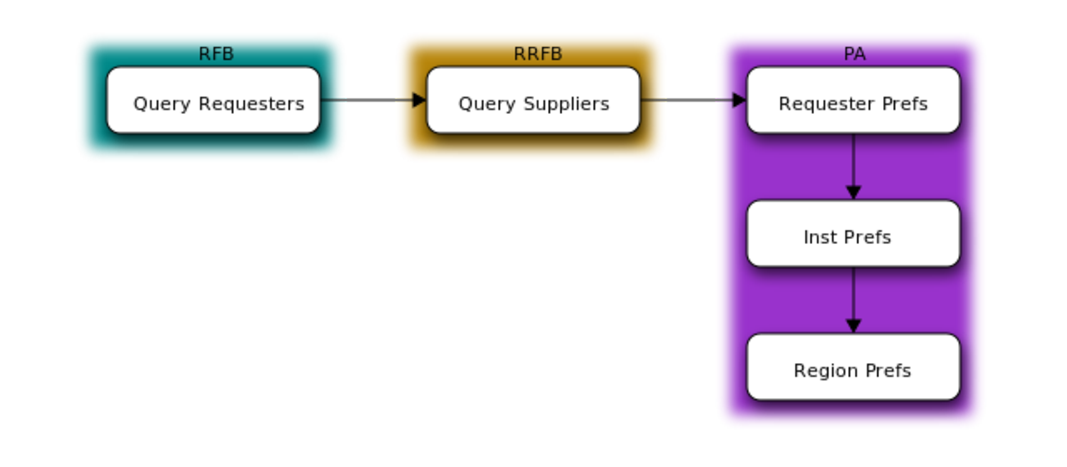
\includegraphics[width=1.2\textwidth]{procedure.pdf}}
  \caption[]{Schematic illustrating the DRE's information
    gathering phases: Request for Bids (RFB), Response to Request for Bids
    (RRFB), and Preference Adjustment (PA).\label{fig:procedure}}
\end{figure}

The first phase allows consumers of commodities to denote both the quantity of a
commodity they need to consume as well as the target isotopics, or quality, by
\textit{posting} their demand to the market exchange. This posting informs
producers of commodities what is needed by consumers, and is termed the
\textit{Request for Bids} (RFB) phase. Consumers are allowed to over-post, i.e.,
request more quantity than they can actually consume, as long as a corresponding
capacity constraint accompanies this posting. Requests can be denoted as
\textit{exclusive}. An exclusive request is one that must either be met in full
or not at all. Exclusive requests allow the modeling of quantized, packaged
transfers, e.g., fuel assemblies. 

Consumers are allowed to post demand for multiple commodities that may serve to
meet the same combine capacity. For example, consider an LWR that can be filled
with MOX or UOX. It can post a demand for both, but must define a preference
over the set of possible commodities that can be consumed. Such requests are
termed \textit{mutual requests}. Another example is that of an advanced fuel
fabrication facility, i.e., one that fabricates fuel partially from separated
material that has already passed through a reactor. Such a facility can choose
to fill the remaining space in a certain assembly with various types of fertile
material, including depleted uranium from enrichment or reprocessed uranium from
separations. Accordingly, it could demand both commodities as long as it
provides a corresponding constraint with respect to total consumption. A set of
exclusive requests may also be grouped as mutual requests, in which case the set
is termed \textit{mutually exclusive}.

At the completion of the RFB phase, the market exchange will have a set of
request \textit{portfolios}. Each each portfolio consists of a set
requests. Arbitrary constraints over the set of requests can be provided that
are functions of quantity or quality.  Each request may have an associated
preference. For requests that mutually satisfy a given demand, a preference
distribution over those requests informs the solver as to which should be
satisfied first, given the constraints. Finally, each request portfolio has a
specific quantity associated with it.

The second phase allows suppliers to \textit{respond} to the set of request
portfolios, and is termed the \textit{Response to Request for Bids} (RRFB) phase
(analogous to Julka's Reply to Request for Quote phase
\cite{julka_agent-based_2002}). Each request portfolio is comprised of requests
for some set of commodities. Accordingly, for each request, suppliers of that
commodity denote production capacities and an isotopic profile of the commodity
they can provide. Suppliers are allowed to offer the null set of isotopics as
their profile, effectively providing no information. Suppliers are also allowed
to denote responses as exclusive, as is done in the RFB phase. Supply responses
can also be grouped into mutual responses, and sets of responses may be mutually
exclusive. This functionality again supports the notion of quantized orders,
e.g., in the case of fuel assemblies. 

A supplier may have its production constrained by more than one parameter. For
example, a processing facility may have both a throughput constraint (i.e., it
can only process material at a certain rate) and an inventory constraint (i.e.,
it can only hold some total material). Further, the facility could have a
constraint on the quality of material to be processed, e.g., it may be able to
handle a maximum radiotoxicity for any given time step which is a function of
both the quantity of material in processes and the isotopic content of that
material. Multiple of such constraints are allowed. At the completion of the
RRFB phase the possible connections between supplier and producer facilities,
i.e., the arcs in the graph of the transportation problem, have been established
with specific capacity constraints defined both by the quantity and quality of
commodities that will traverse the arcs.

The final phase of the information gathering procedure allows consumer
facilities to adjust their set of preferences and for managers of consumer
facilities to affect the consumer's set of preferences. Accordingly, the last
phase is termed the \textit{Preference Adjustment} (PA) phase. By allowing
facility managers, i.e., a facility's institution and region, to also adjust
preferences, socio-economic models are allowed to inform the exchange of
resources. For example, a region can detect a trans-regional trade between one of
its facilities and a facility in another region. If a tariff model is employed,
the trade preference and be diminished or even removed.

For facilities, preference adjustments occurs in response to the set of
responses provided by producer facilities. Consider the example of a reactor
facility that requests two fuel types, MOX and UOX. It may get two responses to
its request for MOX, each with different isotopic profiles of the MOX that can
be provided. It can then assign preference values over this set of potential MOX
providers. Another prime example is in the case of repositories. A repository
may have a defined preference of material to accept based upon its heat load or
radiotoxicity, both of which are functions of the quality, or isotopics, of a
material. In certain simulators, limits on fuel entering a repository are
imposed based upon the amount of time that has elapsed since the fuel has exited
a reactor, which can be assessed during this phase. The time constraint is, in
actuality, a constraint on heat load or radiotoxicity (one must let enough of
the fission products decay). A repository could analyze possible input fuel
isotopics and set the arc preference of any that violate a given rule to 0,
effectively eliminating that arc.

\subsection{The Nuclear Fuel Cycle Transportation Problem}\label{abm:dre:fctp}

Supply and demand in a nuclear fuel cycle context is inherently a multicommodity
problem. A light water reactor can be fueled by both UOX and MOX fuel, for
instance. How it is fueled is a result both of fuel availability and associated
preferences. Allowing for complex physical and chemical constraints on both
processes and inventories, as well as including economics-based approaches for
determining exchange preferences is a complicated affair. Determining the
optimum solution to such a system is even more complicated. Accordingly,
sophisticated tools in both the operations research and agent based modeling
realms have been leveraged to accomplish the task.

An instance of supply and demand defined by the DRE information gathering step
can be solved in a variety of ways. It can be cast to a constrained, bipartite
network, and any heuristic that provides a feasible solution to such networks
are valid. The system can be solved optimally, however, by formulating the
system as a mathematical program. This section describes a Multicommodity
Transportation Problem variant used for this approach, entitled the
\textit{Nuclear Fuel Cycle Transportation Problem} (NFCTP). A linear program
(LP) formulation and a mixed-integer linear program (MILP) formulation are
provided. A greedy heuristic is also designed and implemented.

The LP formulation can be solved quickly, but allows split orders. In other
words, the LP formulation solves a relaxation of the defined instance that does
not take into account \textit{exclusive} requests or bids. The nuclear fuel
cycle deals with bundled orders, such as nuclear fuel assemblies, thus this
modeling paradigm is only an approximation. The MILP provides a more realistic
exchange, but can take much longer to solve. 

\subsubsection{Terminology}

Objects and data structures generated in the information gathering procedure are
used in the formal definition of the NFCTP. Each portfolio can be considered
separately. The set of supply portfolios is denoted as $S$ and the set of
request portfolios is denoted as $R$, and each agent may have multiple
portfolios in a given exchange. Each supply portfolio is comprised of $s_M$
supply nodes, and each request portfolio is comprised of $r_N$ nodes. The set of
supply nodes is denoted $I$, and the set of request nodes is denoted $J$. The
total number of supply and request nodes is then

\begin{equation}
  \left|{I}\right| = \sum_{s \in S} s_M
\end{equation}

and

\begin{equation}
  \left|{J}\right| = \sum_{r \in R} r_N.
\end{equation}

Each portfolio has a set of commodities, $H$, associated with it. These are
denoted $H_s$ for supply portfolios and $H_r$ for request
portfolios. Furthermore, each portfolio has a set of constraints, $K$,
associated with it. Each constraint has a constraining value, $b_s^k$ and
$b_r^k$, respectively. Additionally, each unique combination of portfolio and
constraint has an associated \textit{constraint coefficient conversion
  function}, denoted $\beta_s^k$ for supply portfolios and $\beta_r^k$ for
request portfolios. Each constraint coefficient conversion function takes as an
argument a proposed resource $q_{i,j}$. Request portfolios are provided a
quantity constraint by default for which coefficients are unity. For a set of
\textit{mutual requests}, $M$, where each request has a request quantity, $x_m$,
the coefficient is defined by the ratio between the the average request quantity
over all mutual requests and $x_m$

\begin{equation}
  \beta_{r, m} = \frac{\overline{x_M}}{x_m}.
\end{equation}

The constraint conversion functions are utilized in the NFCTP by applying them
to the proposed resource transfers, creating constraint
coefficients. Coefficients for supply constraints are defined as

\begin{equation}
  a^k_{i, j} = \beta_s^k(q_{i_j}).
\end{equation}

\noindent
Coefficients for request constraints are defined as

\begin{equation}
  a^k_{j, i} = \beta_r^k(q_{i_j}).
\end{equation}

Finally, for each supply-request node pair, there is an associated preference,
$p_{i, j}$. The set of all preferences is denoted $P$. Similarly, flow between a
node pair is denoted $x_{i, j}$, and the set of all flows is denoted $X$. The
possible flow on an arc is provided an upper bound by the request node quantity,
$\widetilde{x_j}$.

\subsubsection{Exchange Graph}

Upon completion of the information gathering phase, a \textit{bipartite} network
is formed which is called an \textit{exchange graph}. The network
consists of sending (bid) nodes, $I$, and receiving (request) nodes, $J$. For
each request node, $j$, there may be many bid nodes; however, there is a
one-to-one mapping between bid nodes and request nodes. In other words, a given
bid node, $i$, is a unique response to a request node, $j$. An example of a bare
exchange graph graph is shown in Figure \ref{fig:ex_bare}.

\begin{figure}
  \begin{center}
    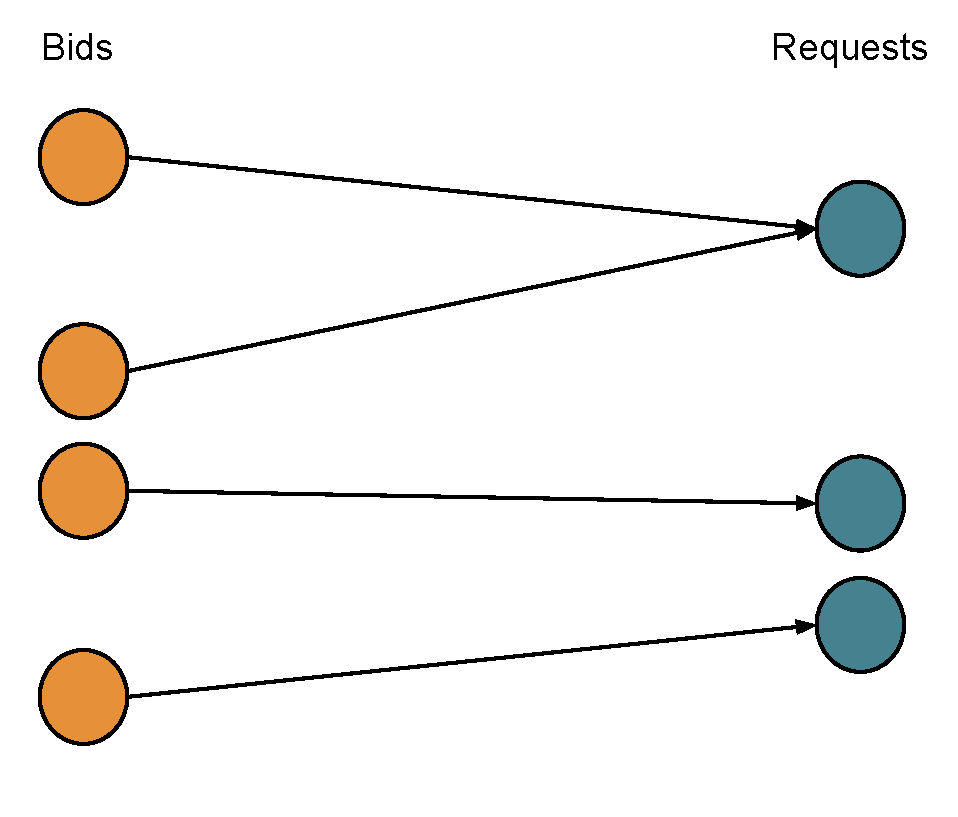
\includegraphics[width=0.75\textwidth]{exchange_bare_words.pdf}
    \caption{A bare example exchange with supply nodes colored orange on left
      and request nodes colored blue on right. As shown, there can be multiple
      supply nodes connected to a request node, but each supply node corresponds
      uniquely to one request node. It is a specific response to that request,
      as outlined in the RRFB phase.}
    \label{fig:ex_bare}
  \end{center}
\end{figure}

In the bipartite graph, portfolios act as partitions that group nodes
together. Node groups share common constraints, and request node groups share a
common notion of satisfiable quantity, i.e., a default mass-based constraint. An
example of a partitioned exchange graph is shown in Figure \ref{fig:ex_groups}.

\begin{figure}
  \begin{center}
    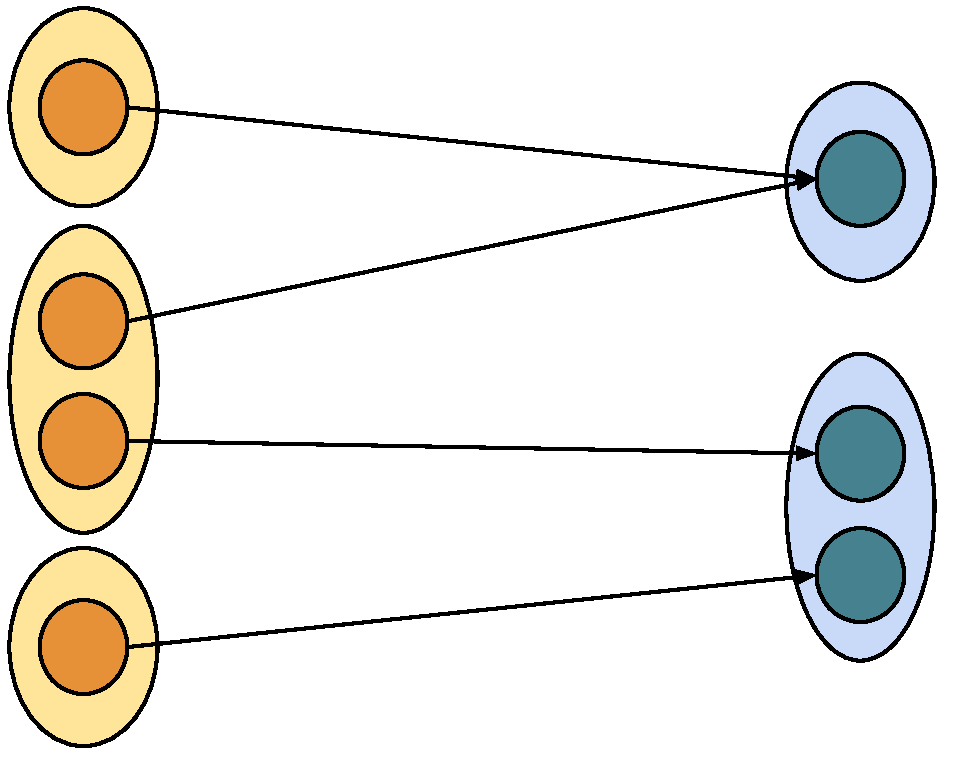
\includegraphics[width=0.75\textwidth]{exchange_groups.pdf}
    \caption{The same exchange shown in Figure \ref{fig:ex_bare} with the
      inclusion of portfolio partitions. In this example, there are three
      supplier agents and two consumer agents. The second consumer has two
      requests (for different commodities) which may satisfy its demand. The
      second supplier can supply the commodities requested by both consumers and
      has provided two bids accordingly.}
    \label{fig:ex_groups}
  \end{center}
\end{figure}

Because of defined constraints, there may not be sufficient supply in the
simulated exchange. To ensure a feasible solution, an unconstrained false supply
node is added to the exchange graph. Additionally, false nodes are added to each
request portfolio and are connected to the false supply source. These arcs are
denoted as \textit{false arcs}. The preferences given to each false arc, $p_f$,
is defined to be lower than the lowest preference in the system, $P$.

\begin{equation}\label{eqn:falsepref}
  p_{f} < \min P
\end{equation}

\noindent
The total number of arcs in the system, $\left|{A_t}\right|$, is then increased
by the number of request portfolios, i.e.,

\begin{equation}
  \left|{A_t}\right| = \left|{A}\right| + \left|{R}\right|
\end{equation}

Because preferences are defined as in Equation \ref{eqn:falsepref}, any false
arc will only be engaged if no other possible arc can be engage, due to capacity
constraints. If any flow is assigned to false arcs after the exchange graph is
solved, that flow is ignored when initiating transactions. Figure
\ref{fig:ex_false} shows a fully defined exchange graph.

\begin{figure}
  \begin{center}
    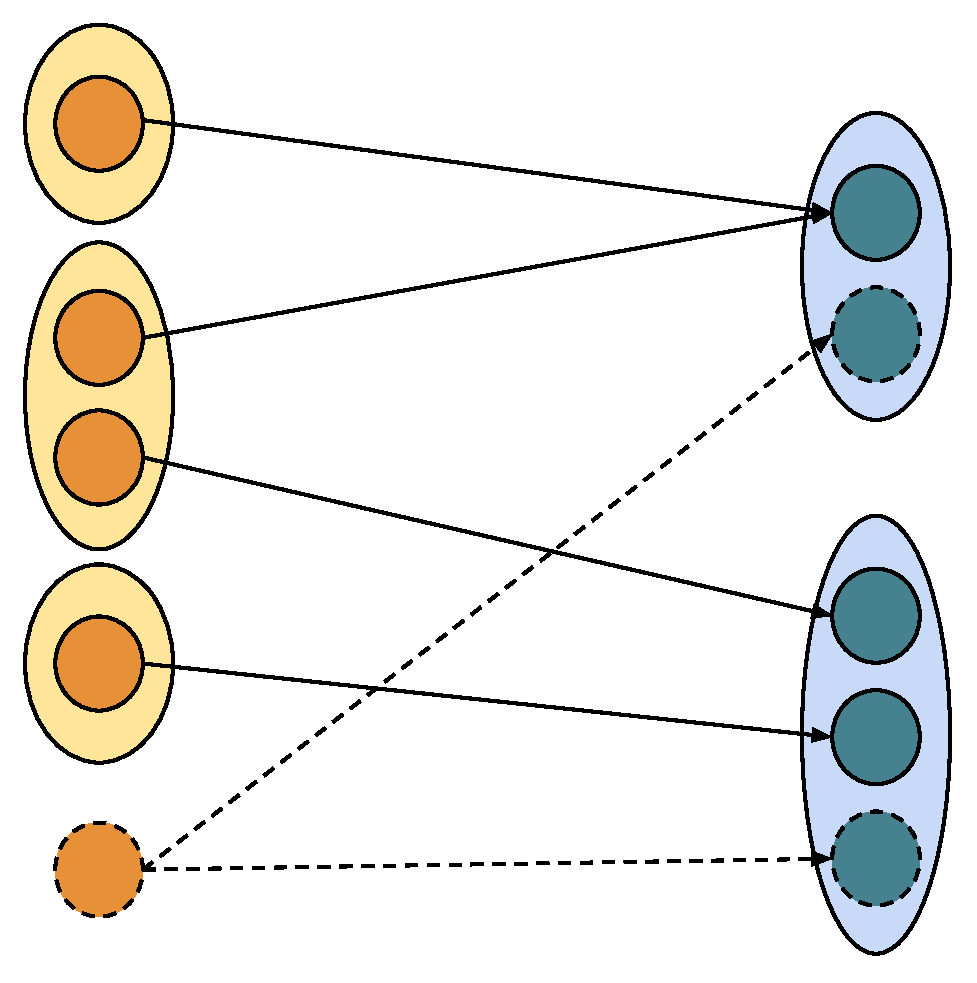
\includegraphics[width=0.75\textwidth]{exchange_false.pdf}
    \caption{The same exchange shown in Figure \ref{fig:ex_groups} with the
      inclusion of false arcs. The false supplier and consumer nodes are shown
      with a dashed outline. Similarly, false arcs are dashed. Note that the
      false nodes have no associated portfolio structure -- there are no
      constraints associated with false nodes and arcs. The inclusion of a false
      supplier and consumer guarantees a feasible solution.}
    \label{fig:ex_false}
  \end{center}
\end{figure}

\subsubsection{Arc Properties}\label{abm:dre:fctp:arcs}

The result of the DRE is flow determined along arcs, where arcs connect supply
nodes to request nodes. A number of properties are defined on arcs, namely
commodities, constraint coefficients, and preferences.

%\paragraph{Commodities}

During the information gathering step in \secref{abm:dre:info}, consumers and
suppliers are queried based on \textit{commodities}. A consumer is allowed to
request multiple commodities, and a supplier is allowed to supply multiple
commodities. However, each possible resource transfer, i.e., each arc, is based
on a single commodity. Accordingly, it is possible to color each arc, given a
commodity-to-color mapping.

For example, consider an exchange similar to that shown in Figure
\ref{fig:ex_groups} with two fuel commodities ($A$, $B$), two requesters ($R_1$,
$R_2$), and two suppliers ($S_1$, $S_2$, $S_3$) in the configuration described
by Tables \ref{tbl:ex_sup} and \ref{tbl:ex_req}.

\begin{table}[h]
\centering
\begin{tabular}{c|c}
Supplier & Commodities \\ \hline
$S_1$             & $A$         \\
$S_2$             & $A$, $B$    \\
$S_3$             & $B$         \\
\end{tabular}
\caption{A mapping from suppliers to commodities supplied.}
\label{tbl:ex_sup}
\end{table}

\begin{table}[h]
\centering
\begin{tabular}{c|c}
Consumer & Commodities \\ \hline
$R_1$             & $A$         \\
$R_2$             & $B$        
\end{tabular}
\caption{A mapping from requesters to commodities requested.}
\label{tbl:ex_req}
\end{table}

Given the color map $A$: green, $B$: brown, the resulting exchange
graph can be colored as shown in Figure \ref{fig:ex_groups_color}.

\begin{figure}
  \begin{center}
    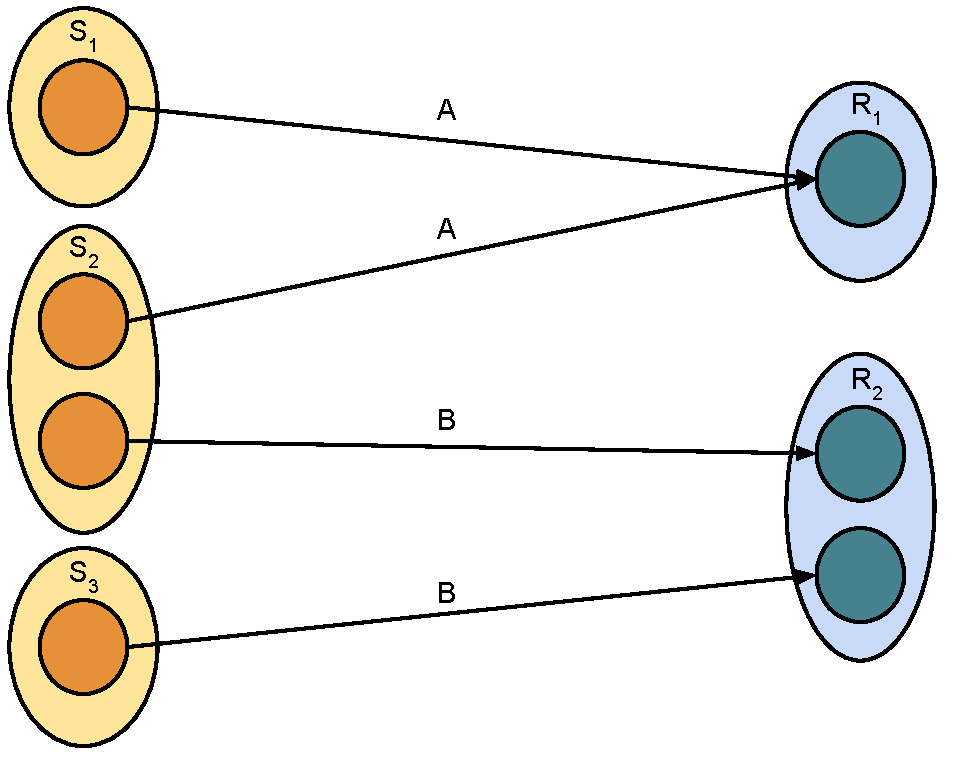
\includegraphics[width=0.75\textwidth]{exchange_groups_color.pdf}
    \caption{The same exchange shown in Figure \ref{fig:ex_groups} arcs colored
      by commodity based on Tables \ref{tbl:ex_sup} and \ref{tbl:ex_req}. A green
      arc corresponds to commodity $A$; a brown arc corresponds to commodity
      $B$.}
    \label{fig:ex_groups_color}
  \end{center}
\end{figure}

The notion of commodities is critical during the information gathering step as
it is the basic classification used in communicating supply and demand. It is
also useful when an exchange graph is formed, because the graph may be able to
be partitioned by collections of commodities. However, once minimally connected
exchange graphs are established, solution mechanisms do not employ the notion of
commodities. Rather, quantities, constraints, and preferences are used.

%\paragraph{Constraint Coefficients}

Constraint coefficients are determined for an arc based on the proposed resource
to be transferred along that arc, the requester's constraint conversion
functions, and the suppliers constraint conversion function. An example of
supply-based constraints is provided to help clarify its purpose.

Consider a supplier enrichment facility, $s$, which produces the commodity
enriched uranium (EU). This facility has two constraints on its operation for
any given time period: the amount of Separative Work Units (SWU) that it can
process, $b_{s}^{SWU}$, and the total natural uranium (NU) feed it has on hand.,
$b_{s}^{NU}$. The constraint set for $s$ is then
 
\begin{equation}\label{eqs:enr-constr-commods}
  K_{s} = \{ \mbox{SWU}, \mbox{NU} \}.
\end{equation}

Note that neither of these capacities are measure directly in the units of the
commodity it produces, i.e., kilograms of EU.

Consider a set of requests for enriched uranium that this facility can possibly
meet. Such requests have, in general, two parameters: $P_{j}$, the total product
quantity (in kilograms), and $\varepsilon_{j}$, the product enrichment (in w/o
\nucl{235}{U}).\footnote{The notation for enrichment, $\varepsilon_{j}$, is
  chosen over its normal form, $x_p$, to limit confusion with the notation of
  material flow, $x^h_{i,j}$.}  For the purposes of this constraint set, the
quality of material in question is its enrichment, i.e.,

\begin{equation}\label{eqs:enr-q-swu}
  q_{j} \equiv \varepsilon_{j}.
\end{equation}

These values are set during a prior phase of the overall matching algorithm, and
can therefore be considered constant. Further, note that, in general, an
enrichment facility's operation, or rather its capacity, is governed by two
parameters: $\varepsilon_{f}$, the fraction of \nucl{235}{U} in its feed
material, and $\varepsilon_{t}$, the fraction of \nucl{235}{U} in its tails
material. These parameters determine the amount of SWU required to produce some
amount of enriched uranium, shown in Equation \ref{eqs:swu} as well as the
amount of natural uranium, or feed, required, as shown in Equation \ref{eqs:nu}.

\begin{align}
\begin{split}
\label{eqs:swu}
SWU = & \:\: P ( V(\varepsilon_{j}) 
      + \frac{\varepsilon_{j} - \varepsilon_{f}}
               {\varepsilon_{f} - \varepsilon_{t}} V(\varepsilon_{t}) \\
      & - \frac{\varepsilon_{j} - \varepsilon_{t}}
               {\varepsilon_{f} - \varepsilon_{t}} V(\varepsilon_{f}) )
\end{split}
\end{align}

\begin{equation}
\label{eqs:nu}
F = P \frac{\varepsilon_{j} - \varepsilon_{t}}
           {\varepsilon_{f} - \varepsilon_{t}}
\end{equation}

\noindent
$P$ in Equations \ref{eqs:swu} and \ref{eqs:nu} is the amount of produced
enriched uranium, $F$ is the amount of feed, or natural uranium, and $V(x)$ is
the value function,

\begin{equation}\label{eqs:value}
  V(x) = (1-2x) \ln \left(\frac{1-x}{x}\right)
\end{equation}

Utilizing the above equations, one can denote the functional forms of the
arguments of this facility's two capacity constraints.

\begin{align}
\label{eqs:enr-prod-beta}
\beta_{s}^{NU}(\varepsilon_{j}) = & \:\: \frac{\varepsilon_{j} - \varepsilon_{t}}
                                      {\varepsilon_{f} - \varepsilon_{t}} \\
\begin{split}
\label{eqs:enr-swu-beta}
\beta_{s}^{SWU}(\varepsilon_{j}) = & \:\: V(\varepsilon_{j}) \\
                         & + \frac{\varepsilon_{j} - \varepsilon_{f}}
                                  {\varepsilon_{f} - \varepsilon_{t}} V(\varepsilon_{t}) \\
                         & - \frac{\varepsilon_{j} - \varepsilon_{t}}
                                  {\varepsilon_{f} - \varepsilon_{t}} V(\varepsilon_{f})
\end{split}
\end{align}

These constraints correspond to the per-unit requirements for enriched uranium
of natural uranium feed and SWU. Finally, we can form the set of constraint
equations for the enrichment facility by combining Equations
\ref{eqs:enr-q-swu}, \ref{eqs:enr-prod-beta}, and \ref{eqs:enr-swu-beta}.

\begin{align}
\label{eqs:enr-prod-constr}
\sum_{j \in J}\beta_{s}^{NU}(\varepsilon_{j}) \: x_{s,j}  & \leq b_{s}^{NU} \\
\label{eqs:enr-swu-constr}
\sum_{j \in J}\beta_{s}^{SWU}(\varepsilon_{j}) \: x_{s,j} & \leq b_{s}^{SWU}
\end{align}

%\paragraph{Preferences \& Costs}

In any network flow problem, of which transportation problems are a subset, the
objective coefficients associated with transporting commodities is what drives
the solution. Given the nature of supply and demand constraints, the
transportation problem naturally lends itself to a minimum cost formulation. A
preference-based formulation has been presented thus far due to the difficulties
of employing reasonable cost coefficients, as was discussed in 
\secref{intro:prefs}. While directly using costs should be available to users, in
practice using a more abstract notion of preferences is simpler.

Formally, a preference function, $p_{i, j}(h)$, is defined which is a cardinal
preference ordering over a consumer's satisfying commodity set.
 
\begin{equation}
p_{i, j}(h) \:\: \forall i \in I  \:\: \forall h \in H_{r} 
\end{equation}

\noindent
A preference is assigned to each arc in the NFCTP, and are a function both of
the consumer, $j$, and producer, $i$, and the proposed resource transfer from
consumer to producer. The dependence on producer encapsulates the relationship
effects due to managerial preferences. The preference set used in the NFCTP
formulation follows directly from the Preference Adjustment phase described in
\secref{abm:dre:info}.

The notion of a preference is a positive one, that is, an optimal solution
maximizes the product of preference and flow in the system. However, the
transportation problem requires a cost-based objective function. Because
preferences are a proxy for cost and there is a desire to support cost-based
DREs in the future, a preference-to-cost translation function is utilized. A
cost translation function, $f$, is defined that operates on the commodity
preference function to produce an appropriate cost for the NFCTP.

\begin{equation}
f : p_{i,j}(h) \to c_{i,j}
\end{equation}

\noindent
For the purposes of this work, any operator that preserves the preference
monotonicity and cardinal ordering is suitable.  The inversion operator has been
chosen because it preserves required features and also allows for easy
translation from preference to cost as well as translation from cost to
preference.

\begin{equation}
f(x) = \frac{1}{x}
\end{equation}

If cost data and a valid cost assignment methodology is developed in the future,
costs may be used directly, and the preference-to-cost translation may be
ignored.

\subsubsection{Linear Programming Formulation}\label{abm:dre:lp}

Combining the previous discussions, the LP Formulation of the NFCTP, denoted the
NFCTP-LP, can be constructed. In general, the NFCTP is a minimum cost
transportation problem that includes custom constraints as described in previous
sections. Including all of the discussion in the previous sections, the
formulation is straightforward and shown in Equation \ref{eqs:NFCTP-LP}.

%%% 
\begin{subequations}\label{eqs:NFCTP-LP}
  \begin{align}
    %%
    \min_{x} \:\: 
    & 
    z = \sum_{i \in I}\sum_{j \in J}c_{i,j} x_{i,j} 
    & 
    \label{eqs:NFCTP-LP_obj} \\
    %%
    \text{s.t.} \:\: 
    &
    \sum_{i \in I_s} \sum_{j \in J} a^k_{i,j} x_{i,j} \leq b^k_s 
    &
    \: 
    \forall \: k \in K_s, 
    \forall \: s \in S 
    \label{eqs:NFCTP-LP_sup} \\
    %%
    &
    \sum_{j \in J_r} \sum_{i \in I} a^k_{i,j} x_{i,j} \geq b^k_r 
    &
    \: 
    \forall \: k \in K_r,  
    \forall \: r \in R 
    \label{eqs:NFCTP-LP_req} \\
    %%
    &
    x_{i,j} \in [0, \tilde{x_j}]
    &
    \forall \: i \in I, 
    \forall \: j \in J 
    \label{eqs:NFCTP-LP_x}
    %%
  \end{align}
\end{subequations}
%%% 

The variables and sets used to define Equation \ref{eqs:NFCTP-LP} have been
described in detail in previous sections. A short synopsis of the sets used is
provided in Table \ref{tbl:NFCTP-LP-sets}, and a corresponding synopsis of the
variables used is provided in Table \ref{tbl:NFCTP-LP-vars}.

%%% 
\begin{table} [h!]
\centering
\begin{tabularx}{\columnwidth-10pt}{|c|X|} % line wraps second column if too long
\hline
Set         & Description \\
\hline
$S$     & suppliers \\
$R$     & requesters \\
$I$     & all supply nodes \\
$I_s$   & nodes for a supplier $s$ \\
$J$     & all request nodes \\
$J_r$   & nodes for a requester $r$ \\
$K_s$   & constraints for a supplier $s$ \\
$K_r$   & constraints for a requester $r$ \\
$X$         & the feasible set of flows between producers and consumers  \\
\hline
\end{tabularx}
\caption{Sets Appearing in the NFCTP-LP Formulation}
\label{tbl:NFCTP-LP-sets}
\end{table}
%%% 

%%% 
\begin{table} [h!]
\centering
\begin{tabularx}{\columnwidth-10pt}{|c|X|} % line wraps second column if too long
\hline
Variable    & Description \\
\hline
$c_{i,j}$             & the unit cost of flow
                          from producer node $i$ to consumer node $j$  \\
$x_{i,j}$             & a decision variable, the flow 
                          from producer node $i$ to consumer node $j$  \\
$a_{i,j}^k$ & the constraint coefficient for constraint $k$ 
                          on flow between nodes $i$ and $j$  \\
$b_s^k$   & the constraining value for constraint $k$ of supplier $s$ \\
$b_r^k$   & the constraining value for constraint $k$ of requester $r$ \\
$\tilde{x_j}$ & the requested quantity associated with request node $j$ \\
\hline
\end{tabularx}
\caption{Variables Appearing in the NFCTP-LP Formulation}
\label{tbl:NFCTP-LP-vars}
\end{table}
%%%

Notably, a feasible solution to the formulation provided in Equation
\ref{eqs:NFCTP-LP} is guaranteed due to the presence of false arcs. Accordingly,
the DRE using this formulation will never fail within a simulation.

\subsubsection{Mixed Integer Linear Programming Formulation}\label{abm:dre:milp}

The previous linear program (LP) formulation of the Generic Fuel Cycle
Transportation Problem fully describes many of the types of transactions that
arise at any given time step. However, it does not allow the critical case of
reactor fuel orders, which comprise a large amount of material orders within the
simulation context. Specifically, it allows reactor fuel orders to be met by
more than one supplier with an arbitrary amount of the order met by each
supplier. Put another way, the LP formulation does not contain the discrete
material information required to model the transaction of fuel assemblies. 

In order to provide this capability of quantizing orders, binary decision
variables must be introduced. The addition of integer variables changes both the
complexity of the formulation and the complexity of the solution technique. Such
a change requires a Mixed Integer-Linear Program (MILP) formulation and solution
via the branch-and-bound method which solves NP-Hard combinatorial optimization
problems.

%\paragraph{Binary Variables}

The primary difference between the LP and MILP formulations is the inclusion
binary decision variables $y_{i,j}$. A variable $y_{i,j}$ has a value of 1 if
flow occurs between producer node $i$ and consumer node $j$. If flow occurs, its
quantity will be equal to the equivalent flow upper bound along that arc,
$\tilde{x}_{j}$, which denote the quantity of a quantized order.

Binary variables, representing quantized flow, are directly related to the
notion of \textit{exclusive} bids and requests discussed in 
\secref{abm:dre:info}. In the MILP formulation, an arc $(i, j)$ is considered
exclusive if either node $i$ or node $j$ was defined as exclusive in the
information gathering phase of the DRE. Accordingly, it is useful to partition
all arcs based on this characteristic. Given the set of arcs $A$, a partition
exists such that $A$ can be separated into exclusive arcs, $A_e$, and
non-exclusive arcs, or arcs that allow partial flow, $A_p$.

\begin{equation}\label{eqs:arc-union}
  A = A_{p} \cup A_{e}
\end{equation}

Similarly, each partition can be further subdivided into partitions based on
supplier and requester. 

\begin{equation}\label{eqs:arc-union}
  A = \bigcup_{r \in R} A_{p_r} \cup A_{e_r}
\end{equation}

\begin{equation}\label{eqs:arc-union}
  A = \bigcup_{s \in S} A_{p_s} \cup A_{e_s}
\end{equation}

%\paragraph{Mutually Exclusive Constraints}

\textit{Mutual} requests and responses were described in 
\secref{abm:dre:info}. These are defined as a set of requests or responses, of
which only one may be satisfied. This is represented in the formulation as a
constraint on the associated variables. Again, if a variable $y_{i,j}$ is set to
$1$, flow is sent along arc $(i, j)$. If it is $0$, no flow occurs. A
\textit{mutually exclusive} constraint simply says that only one arc in a mutual
set may have a value of 1.

The set of mutually satisfying arcs is denoted $M_s$ and $M_r$ for suppliers and
requesters, respectively. The associated constraints are then defined by
Equations \ref{eqs:mutual_sup} and \ref{eqs:mutual_req}.

\begin{equation}\label{eqs:mutual_sup}
  \sum_{(i, j) \in M_{s}} y_{i,j} \leq 1 \: \forall \: s \in S 
\end{equation}

\begin{equation}\label{eqs:mutual_req}
  \sum_{(i, j) \in M_{r}} y_{i,j} \leq 1 \: \forall \: r \in R 
\end{equation}

%\paragraph{Formulation}

Using the above arc partition notation allows for a much simpler written
formulation of the MILP that looks quite close to the related LP formulation
shown in Equation \ref{eqs:NFCTP-LP}. The full formulation of the NFCTP is shown
in Equation \ref{eqs:NFCTP}.  The sets and variables involved in Equation
\ref{eqs:NFCTP} are described in Tables \ref{tbl:NFCTP-sets} and
\ref{tbl:NFCTP-vars}.


%%% 
% this could probably be realigned 
\begin{subequations}\label{eqs:NFCTP}
  \begin{align}
    %%
    \min_{x, y} \:\: 
    & 
    z \:\: = 
    \sum_{(i, j) \in A_p} c_{i,j} x_{i,j} 
    \: + 
    \sum_{(i, j) \in A_e} c^{\prime}_{i,j} y_{i,j} 
    & 
    \label{eqs:NFCTP_obj} \\
    %%
    \text{s.t.} \:\: 
    &
    \sum_{(i, j) \in A_{p_s}} a^k_{i,j} x_{i,j}
    \: + 
    \sum_{(i, j) \in A_{e_s}} a^{k\prime}_{i,j} y_{i,j}
    \leq b^k_s 
    &
    \: 
    \forall \: k \in K_s, 
    \forall \: s \in S 
    \label{eqs:NFCTP_sup} \\
    %%
    &
    \sum_{(i, j) \in M_{s}} y_{i,j} \leq 1 
    &
    \forall \: s \in S 
    \label{eqs:NFCTP_mut_sup} \\
    %%
    &
    \sum_{(i, j) \in A_{p_r}} a^k_{i,j} x_{i,j}
    \: + 
    \sum_{(i, j) \in A_{e_r}} a^{k\prime}_{i,j} y_{i,j}
    \geq b^k_r 
    &
    \: 
    \forall \: k \in K_r,  
    \forall \: r \in R 
    \label{eqs:NFCTP_req} \\
    %%
    &
    \sum_{(i, j) \in M_{r}} y_{i,j} \leq 1 
    &
    \forall \: r \in R 
    \label{eqs:NFCTP_mut_req} \\
    %%
    &
    x_{i,j} \in [0, \tilde{x_j}]
    &
    \forall \: (i, j) \in A_p
    \label{eqs:NFCTP_x} \\
    %%
    &
    y_{i,j} \in \left\{ 0, 1 \right\}
    &
    \forall \: (i, j) \in A_e
    \label{eqs:NFCTP_y}
    %%
  \end{align}
\end{subequations}
%%% 

\noindent
The above formulation uses a simplified representation of constraint
coefficients for binary variables shown in Equation \ref{eqs:constr_simple} and
objective coefficients shown in Equation \ref{eqs:obj_simple}.

\begin{equation}\label{eqs:constr_simple}
a^{k\prime}_{i,j} = a^k_{i,j} \tilde{x_j}
\end{equation}

\begin{equation}\label{eqs:obj_simple}
c^{\prime}_{i,j} = c_{i,j} \tilde{x_j}
\end{equation}

%%% 
\begin{table} [h!]
\centering
\begin{tabularx}{\columnwidth-10pt}{|c|X|} % line wraps second column if too long
\hline
Set         & Description \\
\hline
$S$     & suppliers \\
$R$     & requesters \\
$A_p$     & arcs that allow \textit{partial} flows \\
$A_e$     & \textit{exclusive} flow arcs  \\
$A_{p_s}$     & arcs that allow \textit{partial} flows for supplier $s$ \\
$A_{e_s}$     & \textit{exclusive} flow arcs for supplier $s$ \\
$A_{p_p}$     & arcs that allow \textit{partial} flows for requester $r$ \\
$A_{e_p}$     & \textit{exclusive} flow arcs for requester $r$ \\
$M_s$     & arcs $(i, j)$ associated with \textit{mutually exclusive} supply for supplier $s$ \\
$M_r$     & arcs $(i, j)$ associated with \textit{mutually exclusive} requests for requester $r$ \\
$X$         & the feasible set of flows between producers and consumers  \\
$Y$         & the binary variable set of flows between producers and consumers  \\
\hline
\end{tabularx}
\caption{Sets Appearing in the NFCTP Formulation}
\label{tbl:NFCTP-sets}
\end{table}
%%% 

%%% 
\begin{table} [h!]
\centering
\begin{tabularx}{\columnwidth-10pt}{|c|X|} % line wraps second column if too long
\hline
Variable    & Description \\
\hline
$c_{i,j}$             & the unit cost of flow
                          from producer node $i$ to consumer node $j$  \\
$x_{i,j}$             & a decision variable, the flow 
                          from producer node $i$ to consumer node $j$  \\
$y_{i,j}$             & a decision variable, whether flow exists 
                          from producer node $i$ to consumer node $j$  \\
$a_{i,j}^k$ & the constraint coefficient for constraint $k$ 
                          on flow between nodes $i$ and $j$  \\
$b_s^k$   & the constraining value for constraint $k$ of supplier $s$ \\
$b_r^k$   & the constraining value for constraint $k$ of requester $r$ \\
$\tilde{x_j}$ & the requested quantity associated with request node $j$ \\
\hline
\end{tabularx}
\caption{Variables Appearing in the NFCTP Formulation}
\label{tbl:NFCTP-vars}
\end{table}
%%%

The examples of the various constraints from the previous section also apply
here. The only difference is the notion of the binary variables, $y_{i,j}$,
which act as on/off switch as to whether a consumer's entire requested amount of
a resource is met by a supplier or not. 

Using this advanced formulation adds significant complexity to the resolution
method at every time step. However, should a user wish to find a feasible
solution in a shorter amount of time, simple heuristics exist. Such a heuristic
used in Cyclus is provided in \secref{abm:dre:nfctp:heur}, and further heuristic
development is a fruitful area of future work.

%%% 
% this could probably be realigned 
%%% 

\subsubsection{A Heuristic Solution}\label{abm:dre:nfctp:heur}

With full simulation domain knowledge of supply and demand, including false
arcs, a feasible solution can be found. By definition a feasible solution is a
\textit{solution} to the possible flow of resources, but not necessarily an
\textit{optimal} solution. Many heuristics may be applied to bipartite graphs
with constrained flows. A simple \textit{greedy} heuristic is presented here
and implemented. 

The maximum flow along an arc, $x_{max}$, depends on the constraints associated
with each node on the arc. For nodes $i$ and $j$ belonging to portfolios $s$ and
$r$, respectively, the maximum allowable flow is defined as

\begin{equation}
  x_{max} = \min 
        \lbrace 
        \min \lbrace \frac{b^k_s}{a^k_{i, j}} 
        \: \forall k \in K_s \rbrace, 
        \: \min \lbrace \frac{b^k_r}{a^k_{i, j}} 
        \: \forall k \in K_r \rbrace
        \rbrace.
\end{equation}

The Greedy Exchange Heuristic matches maximum flow along arcs, up to the
requested amount defined by each request portfolio, $q_r$, after having sorted
all arcs. The constraining values of each arc, $b_k$, are updated upon
declaration of a match (via an \code{AddMatch} function) in Algorithm
\ref{alg::greedy}.

\begin{algorithm}[!h]
 \SetAlgoLined
 \KwData{A resource exchange graph with constraints and preferences.}
 \KwResult{A valid set of resource flows.}
 sort request partitions by average preference\;
 \ForAll{$r \in R$} {
   sort requests by average preference\;
   matched $\leftarrow$ 0\;        
   \While{matched $\leq q_r$ and $\exists$ a request} {
     get next request\;
     sort incoming arcs by preference\;
     \While{matched $\leq q_r$ and $\exists$ an arc} {
       get next arc\;
       remaining $\leftarrow q_r$ - matched\;
       to\_match $\leftarrow \min \lbrace$remaining, $x_{max} \rbrace$\;
       \code{AddMatch}(arc, to\_match)\;
       matched $\leftarrow$ matched + to\_match\;
     }
   }
 }
 \caption{Greedy Exchange Heuristic}\label{alg::greedy}
\end{algorithm}

\subsubsection{Departure from the MCTP}

The classic MCTP includes the coloring of flows based on commodity type. For
example, for a commodity, $h$, the unit cost of flow would be $c^h_{i,j}$ rather
than $c_{i, j}$. This is included because multiple commodities can flow along
the same arc in the MCTP. In other words, the node-arc incidence matrix includes
an extra commodity dimension. 

The multicommodity nature of the NFCTP is included in constraints, rather than
arcs. Because each node pairing, $(i, j)$, corresponds to a specific, proposed
resource transfer, it can only have one commodity associated with it. Instead,
the constraint set, $K$, is applied over multiple arcs, where each arc is
assigned its own commodity. 

Take the enrichment facility example, expanding on the previous discussion. Note
that an enrichment facility takes feed uranium and then enriches its
\nucl{235}{U} content. This feed uranium can come from different sources which
have different feed enrichments. In practice, the most likely sources of feed
uranium are natural uranium (NU) or recycled uranium (RU), a product of
reprocessing light water reactor fuel. Recycled uranium may be advantageous to
use if it has a higher weight percent of \nucl{235}{U} than does natural
uranium. We can now state the set the values for $H_{r}$ for this facility:

\begin{equation}\label{eqs:enr-dem-commods}
  H_{r} = \{ \mbox{NU}, \mbox{RU} \}
\end{equation}

\noindent
One or more constraints would then accompany any requests. For example, one
could constraint total \nucl{235}{U} content needed, which would include both NU
and RU flows.

\subsection{Implementation}\label{abm:dre:impl}

The DRE and its solution framework are implemented in three layers. The first
layer includes information for specific \code{Resource} types. For example, a
\code{Material}-based exchange is used for agents to communicate supply and
demand information regarding \code{Material} objects. The \textit{resource
  layer} is the point of entry and exit of the DRE framework. It is the
agent-facing interface of the DRE: supply and demand is provided to the DRE as
input during the information gathering step, and trades to be executed are
provided to agents as output.

The second layer, called the \textit{exchange layer}, is a
\code{Resource}-agnostic implementation of a specialized bipartite
graph. Supply/demand constructs in the first layer are translated into stateful
objects representing nodes, arcs, constructs that carry constraint information,
\textit{et cetera}. The collection of objects and structures combine to create
an \code{ExchangeGraph}. Any custom, Cyclus-aware solver can be applied to an
\code{ExchangeGraph} to determine a feasible solution to the DRE.

In order to use sophisticated, 3\textsuperscript{rd} party LP and MILP solving
libraries, the \code{ExchangeGraph} must be translated into an appropriate data
structure representing an instance of the NFCTP, resulting in the
\textit{formulation layer}. The Open Solver Interface (OSI) \cite{coinosi} is
used to create the necessary formulation structures, including a constraint
matrix and objective coefficient vector. The NFCTP instance is then solved.

After a feasible, perhaps optimal, solution to the NFCTP is found, whether in
the exchange or formulation layer, the solution is back-translated to the
resource layer. The agents associated with successful supply-demand connections
are informed, and trades of resources between agents are executed. A graphic of
the entire workflow is shown in Figure \ref{fig:dre_impl}.

\begin{figure}
  \begin{center}
    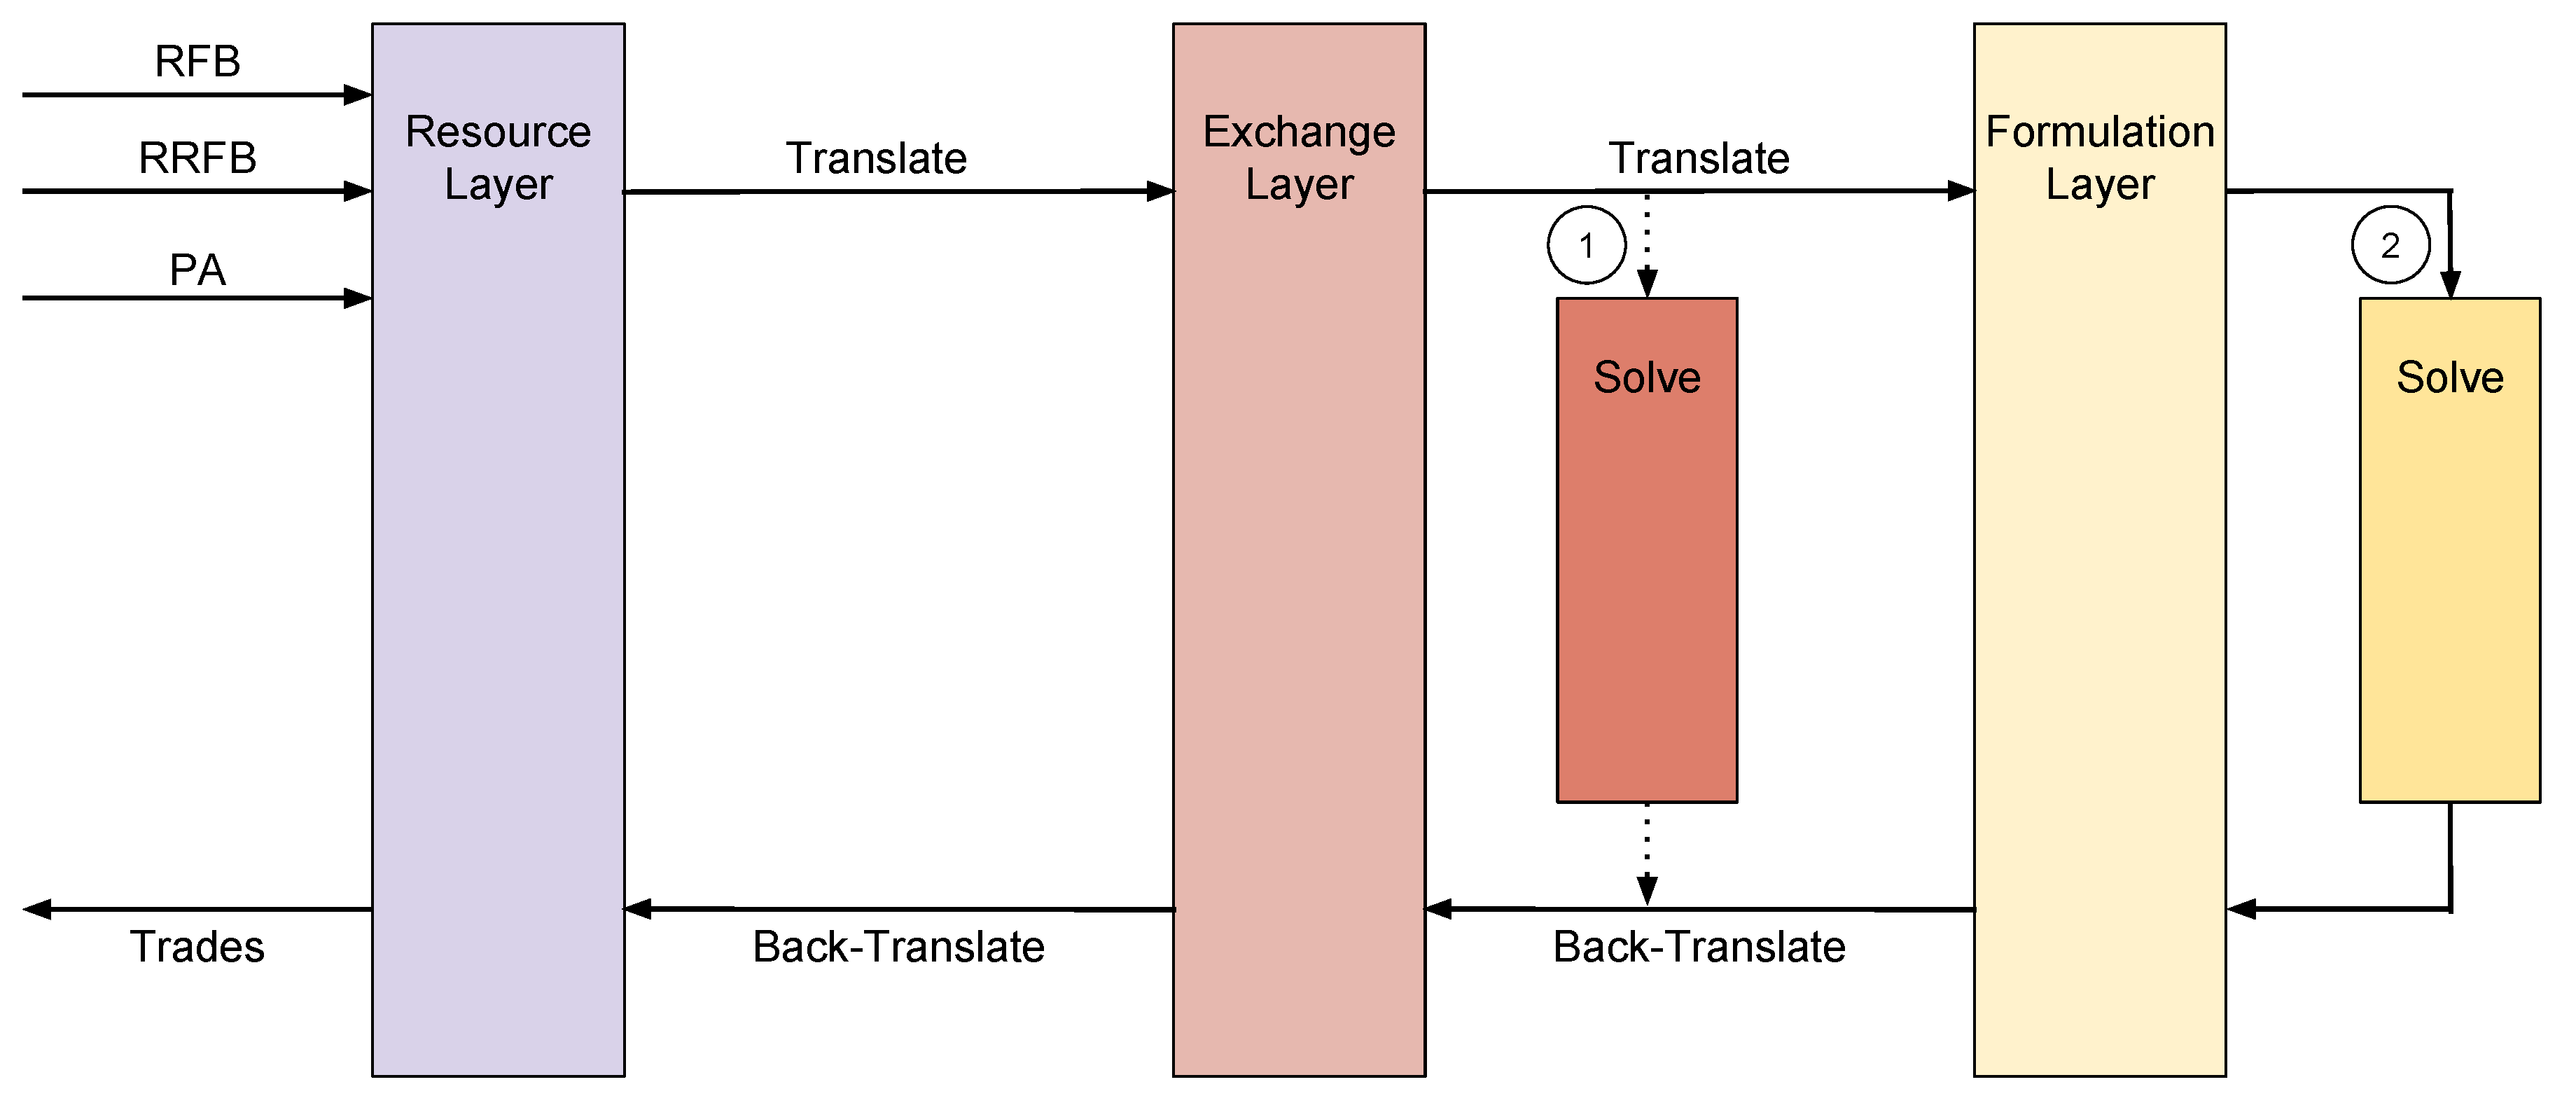
\includegraphics[width=\textwidth]{exchange_xlation.pdf}
    \caption[]{
      \label{fig:dre_impl}
      The full DRE workflow is shown. The information gathering phase results in
      the resource layer. The resource layer is translated to the exchange
      layer; a decision is made whether to continue translation or to directly
      solve, marked by the number $1$. If the exchange is not solved, it is
      translated into an instance of the NFCTP resulting in the formulation
      layer. A choice of solver is made, marked by the number $2$, and the
      instance is solved.  The solution is back-translated through the exchange
      and resource layers. The result is a series of resource trades to be
      executed in the simulation.}
  \end{center}
\end{figure}

\subsubsection{Resource Layer}

The resource layer utilizes \textit{templated} classes in order to reduce the
amount of code required for implementation. Each object is templated on the
concrete \code{Resource} type, e.g., the \code{Material} and \code{Product}
classes. The fundamental data structures in the resource layer reflect the
constructs of the information gathering procedure described in 
\secref{abm:dre:info}.

In the RFB phase of the DRE, agents populate \codeb{Request\-Portfolio}s with
\code{Request}s and \codeb{Capacity\-Constraint}s. A \code{Request}
defines a desired \code{Resource}, communicating quantity, quality, and
preference. Any number of \codeb{Capacity\-Constraint}s may be added to a
\codeb{Request\-Portfolio}. A \codeb{Capacity\-Constraint} defines a
capacitating value and a conversion function that takes as an argument a
\code{Resource} and returns a value in units of the conversion function. For
\codeb{Request\-Portfolio}s, constraints are assumed to be demand
constraints, i.e., take the form of a greater-than constraint. In the RRFB phase
of the DRE, agents populate \codeb{Bid\-Portfolio}s with \code{Bid}s and
\codeb{Capacity\-Constraint}s. Agents can inspect the population of
\code{Request}s and associated \code{Resource}s. A \code{Bid} targets a
specific \code{Request}, responding with a proposed \code{Resource} to
transfer to the requester. \codeb {Capacity\-Constraint}s are applied to all
\code{Bid}s in a portfolio. For bidders, constraints are assumed to be
less-than constraints. Before continuing, requesting agents and their managers
are allowed to alter the preference associated with each
\code{Request}-\code{Bid} pair in the PA phase of the DRE. When a solution
to the DRE is found, bidders associated with successful
\code{Request}-\code{Bid} pairs are informed, and a trade of the bidder's
\code{Resource} is initiated.

Future work can be focused on providing more features to the DRE
implementation. A natural extension of the present work is to support both kinds
of constraints, greater and less-than, in \code{Portfolio} data
structures. Additionally, the PA procedure could use a negotiation model that
involves both suppliers and requesters in order to define a final preference for
an arc. Such an extension would allow for more seamless and natural usage of arc
costs in addition to preferences.

\subsubsection{Exchange Layer} 

The exchange layer is constructed by an \code{ExchangeTranslator} object that
translates the resource layer objects into an instance of an
\code{ExchangeGraph}. Request and bid objects are translated to
\code{ExchangeNode}s, and portfolio objects are translated to
\code{ExchangeGroup}s. Constraint coefficient and preference information is
recorded on \code{ExchangeArc}s, which store a reference to a supply
\code{ExchangeNode} and a demand \code{ExchangeNode}. Finally, constraint values
are stored on the appropriate \code{ExchangeGroup} object.

An \code{ExchangeContext} object is tasked with storing a mapping from
\code{Request} and \code{Bid} objects to their associated
\code{ExchangeNode}. Importantly, the exchange layer does \textit{not} depend on
resource type, i.e., the resource type is abstracted away during
translation. Finally, a general solver can be implemented that operates on the
\code{ExchangeGraph}. A solution to the \code{ExchangeGraph} instance is a
mapping from \code{ExchangeArc}s to flow quantities that does not violate the
provided constraints. After a solution is found, it is back-translated to the
resource layer.

\subsubsection{Formulation Layer}

While a solver may operate on the exchange layer, an instance of an
\code{ExchangeGraph} can be translated fully into the NFCTP. Once in an LP or
MILP form, the DRE instance can be solved by sophisticated 3\textsuperscript{rd}
party libraries. In order to interface with a large number of the possible
solvers, including COIN-OR and CPLEX, the COIN-OR OSI API \cite{coinosi} is
utilized.

The translation from the exchange layer to formulation layer is managed by the
\code{ProgTranslator} class. A variable in the NFCTP is associated with each
\code{ExchangeArc}, with variable bounds set by request values on
\code{ExchangeNode}s; a binary variable is used if the arc is exclusive,
otherwise a linear variable is used. Capacity coefficients and preference values
defined for \code{ExchangeArc}s are translated into an objective coefficient
vector and constraint matrix. The right-hand-side $b$ constraint vector is
determined by \code{ExchangeGroup} constraining values.

A solution to the NFCTP instance is determined by the identified solver,
assigning values to linear and integer variables. Linear variable values map
directly to assigned resource flow quantity. If a binary variable is set to
unity in a solution, the maximum possible flow value is assigned, analogous to
$\tilde{x_j}$ in the NFCTP formulation. The variable-flow value assignment is
then back-translated into an equivalent \code{ExchangeArc}-flow value assignment
by the \code{ProgTranslator}.

\subsection{Inter-region Policy Instruments}\label{meth:tariff}

Modeling international fuel cycles requires a simulator to support a notion of
regional boundaries. To date, DESAE is the only simulator to advertise such a
feature, providing static models of regional relationships as input
\cite{andrianova_desae_2008}. Accordingly, no NFC simulator provides any
representation dynamic models of inter-region policy instruments, such as
tariffs.

\Cyclus natively supports inter-regional flows via its
Region-Institution-Facility hierarchy \cite{huff_cyclus_2015}. While the DRE is
capable of \textit{supporting} dynamic relationship models through its
preference adjustment phase, no such models have heretofore been
implemented. The only flow-based relationship models currently offered occur at
the facility level. That is, certain facilities may set commodity-based
preferences for potential material flows. For example, a \texttt{Reactor}
prototype may set its preference for MOX-based fuels higher than UOX-based
fuels, and the DRE will provide it with MOX-based fuels if it is able.

A new \texttt{Region} archetype has been developed to explicitly support both
static and dynamic inter-region policy instrument models
\cite{tariff_region_doi}. Named the \texttt{TariffRegion}, it applies instrument
models, such as tariffs, during the preference-adjustment phase of the DRE
according to a given \textit{rule}. Rules may be applied, updated, and removed
as a function of time, thereby supporting dynamic instrument models. Static
models are trivially supported by applying a rule at the initial time step and
not removing it.

Rules are comprised of \textit{conditions} and \textit{tariffs}. Given a
condition and tariff, preferences are adjusted as shown in Algorithm
\ref{alg::tariff}.

\begin{algorithm}[!h]
 \SetAlgoLined
 \KwData{A potential trade, a condition, and a tariff value, $x$.}
 \KwResult{An updated preference value, $p$.}
 \eIf{trade meets condition}{return $p * x$}{return $p$}
 \caption{\texttt{TariffRegion} Preference Adjustment}\label{alg::tariff}
\end{algorithm}

A rule's condition may depend on any factor that is queryable during the
preference adjustment phase of the DRE. During PA, each potential resource
transfer is known. Therefore, rules may depend on information regarding the
supplier or consumer (e.g., in which region each resides), the commodity
associated with the transfer, and both the resource quantity and quality (e.g.,
the fissile plutonium content for material resources). 

At present, the \texttt{TariffRegion} supports region-based rules. Each rule
applies to another region. The rule's condition is met if the opposing facility
involved in the trade is in the associated region. If so, a tariff, value is
applied, per Algorithm \ref{alg::tariff}.


\section{Experimentation \& Results}\label{sec:results}


A number of computational experiments are conducted to highlight unique features
enabled by the DRE in Cyclus. Each experiment is performed by solving instances
of the DRE using both the \greedy heuristic and to optimality with the
branch-and-bound solver \cbc. A UOX-MOX one-pass recycle system with all
required fuel cycle facilities is taken as the \basecase scenario in order to
reduce the complexity of the fuel cycle and highlight departures from available
simulators. For simplicity of demonstration, reactors are assumed to refuel
completely with a single commodity rather than a combination of fuel types as is
done in practice. A simulation time frame of 50 years is chosen with one-month
time-steps (totaling 600 simulation time steps), sufficient to display all
relevant effects. The nominal parameters of all common facilities in the
simulation are shown in \cite{gidden_dre_2016}.

The \basecase scenario is not process constrained (i.e., it is constrained only
by the dynamics of Pu availability in the recycling stream). Reactors are
allowed to be fueled by either UOX or MOX, with a preference for MOX over UOX,
and refuel one-third of their total core mass every 18 months. Spent UOX fuel is
allowed to be recycled, whereas spent MOX fuel is sent directly to a
repository. In order to involve dynamism in the simulation, the population
reactors grows linearly over time at a rate of 1 reactor every 5 years. An
initial population of 20 reactors are deployed individually in each of the first
20 time-steps of the simulation as shown in Figure \ref{fig:deploy}. Note that
deployments are staggered in the initial period in order to avoid supply/demand
clustering effect. A diagram of the full \basecase fuel cycle is shown in Figure
\ref{fig:base}.

\begin{figure}
  \begin{center}
    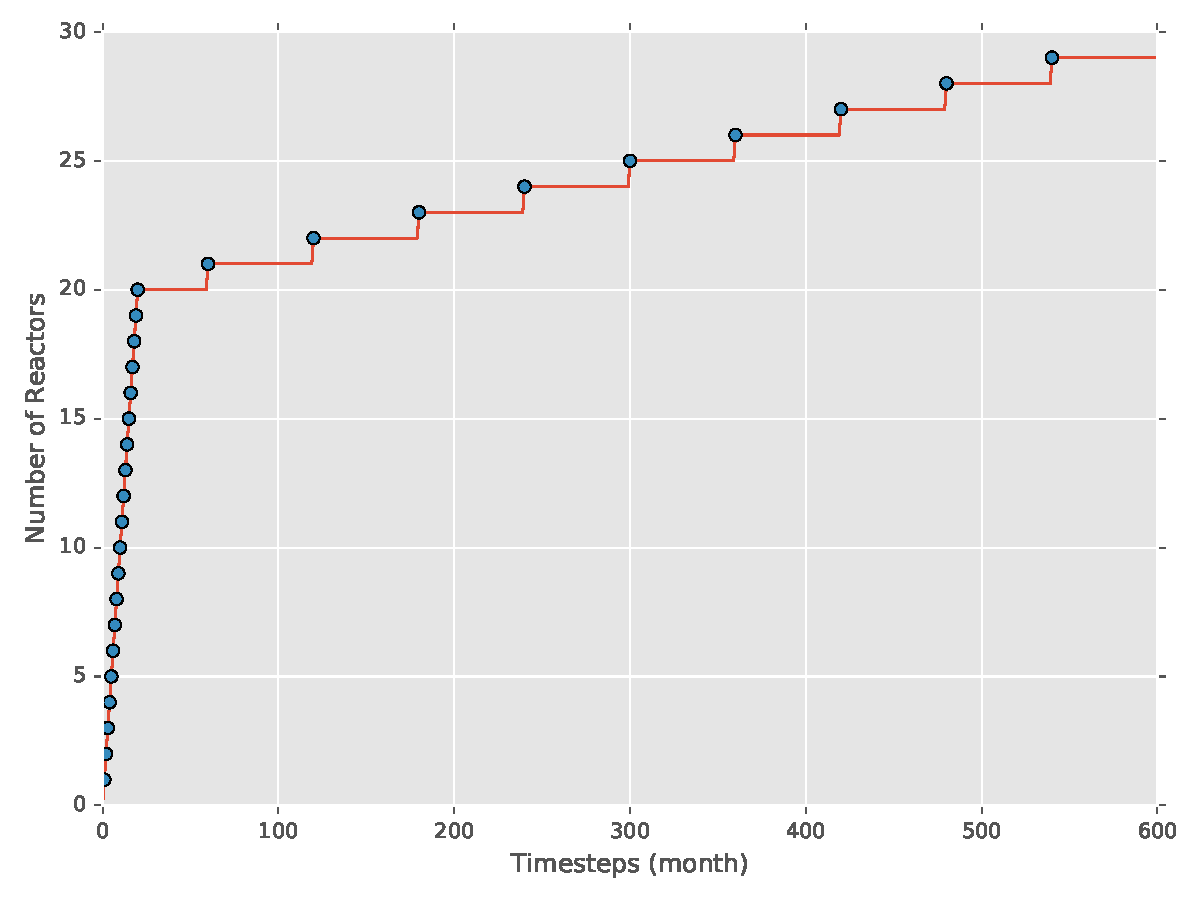
\includegraphics[width=\columnwidth]{rxtr_deploy.pdf}
    \caption[]{
      \label{fig:deploy}
      \reactor deployment in each simulation as a function of simulation time
      steps. Each point in the graph is a reactor being deployed in the
      simulation. Deployments for the \tariff scenario are distinguished by
      color: blue represents deployments in Region A and purple represents
      deployments in Region B.}
  \end{center}
\end{figure}

\begin{figure}
  \begin{center}
    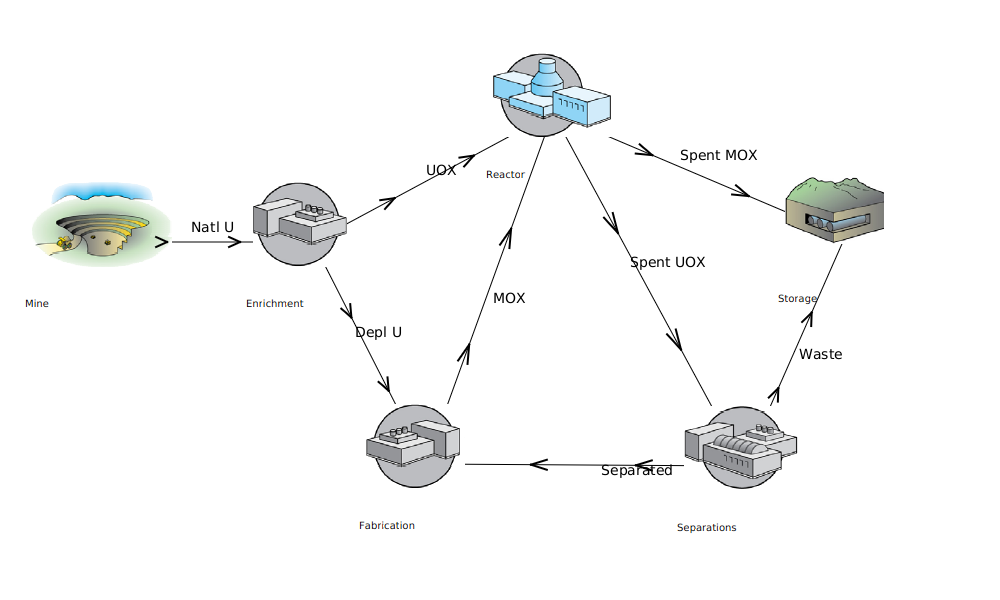
\includegraphics[width=\columnwidth]{base_case_fc}
    \caption[]{
      \label{fig:base}
      Material routing between in the \basecase scenario, single-pass MOX fuel
      cycle. Possible arc flows are labeled with commodity names.}
  \end{center}
\end{figure}

Three perturbations from the \basecase scenario are used to provide examples of
modeling capability enabled through the use of the DRE. The scenarios are
summarized in Table \ref{scenarios} below and described in more detail in the
following sections. 

\begin{table}[]
\centering
\caption{Short Descriptions of Scenarios Ran}
\label{scenarios}
\begin{tabularx}{\textwidth}{|p{1.5cm}|p{1.5cm}|X|X|}
\hline
\textbf{Scenario  Name} & \textbf{Scenario Handle} & \textbf{Primary Departure from Base Case}                & \textbf{Capability Highlighted}                             \\ \hline
Separations Outage      & \outage                   & Separations facility halts operation mid-simulation      & System flexibility to recycling facilities operation        \\ \hline
External MOX Supplier   & \external                 & An additional supplier of MOX enters mid-simulation      & System flexibility to entry and exit of commodity suppliers \\ \hline
Regional Tariffs        & \tariff                   & Two regions are modeled with dynamic trade relationships & Ability to model nontrivial international relationships     \\ \hline
\end{tabularx}
\end{table}

\subsection{Separations Outage: Fuel Cycles with Supply Disruption}

The DRE provides a unifying framework in which any instance of supply and demand
can be formulated and solved. This flexibility lends itself well to dynamic
simulation in which the state of actors in a simulation, by definition, can
change as the simulation progresses. In order to show case the types of
simulations that are enabled by this feature, a fuel cycle simulation is
constructed that has multiple types of reactor fuel input and a defined supply
disruption within the recycled-fuel supply chain.

The chosen disruption is an outage of the separations facility shown in Figure
\ref{fig:base}. The outage begins at $t_i = 250$, lasts 50 time steps, ending at
$t_f = 300$. During the outage, the remaining facilities in the supply chain
operate normally, and the flow of fuel into and out of reactors adapts according
to the state of available fresh fuel. Importantly, neither the \separations or
\fabrication facilities have throughput constraints, i.e., both facilities are
immediately able to process any quantity of fuel.

A comparison of the inventories of plutonium (Pu) in each facility type of
interest among the \basecase and \outage scenarios is shown in Figure
\ref{fig:outage}. As can be seen in Figure \ref{fig:baseinv-outage}, the
quantity of MOX in \reactors is under a dynamic equilibrium, oscillating between
the maximum quantity allowable in the system and one refueling quantity less
than the maximum, based on refueling schedules. The equilibrium value increases
in a stair-step-function manner as the number of reactors increases to being
able to provide sufficient used UOX for the next marginal refueling quantity of
MOX. The quantity of MOX in \fabrication oscillates between a minimal value and
a maximum value which is sufficient for a single reactor's refueling
quantity. As soon as there is sufficient MOX fuel for another refueling
\textit{and} a reactor makes a request to be refueled, it is provided the
quantity of MOX in of fresh fuel. Finally, \separations separates the various
actinides of used fuel and passes on fissile isotopes to \fabrication, thus
maintaining a small oscillating inventory in each timestep.

\begin{figure}
  \centering
  \begin{minipage}{0.67\textwidth}
    \centering 
    \subfloat[Pu inventories in the \basecase scenario.]{
      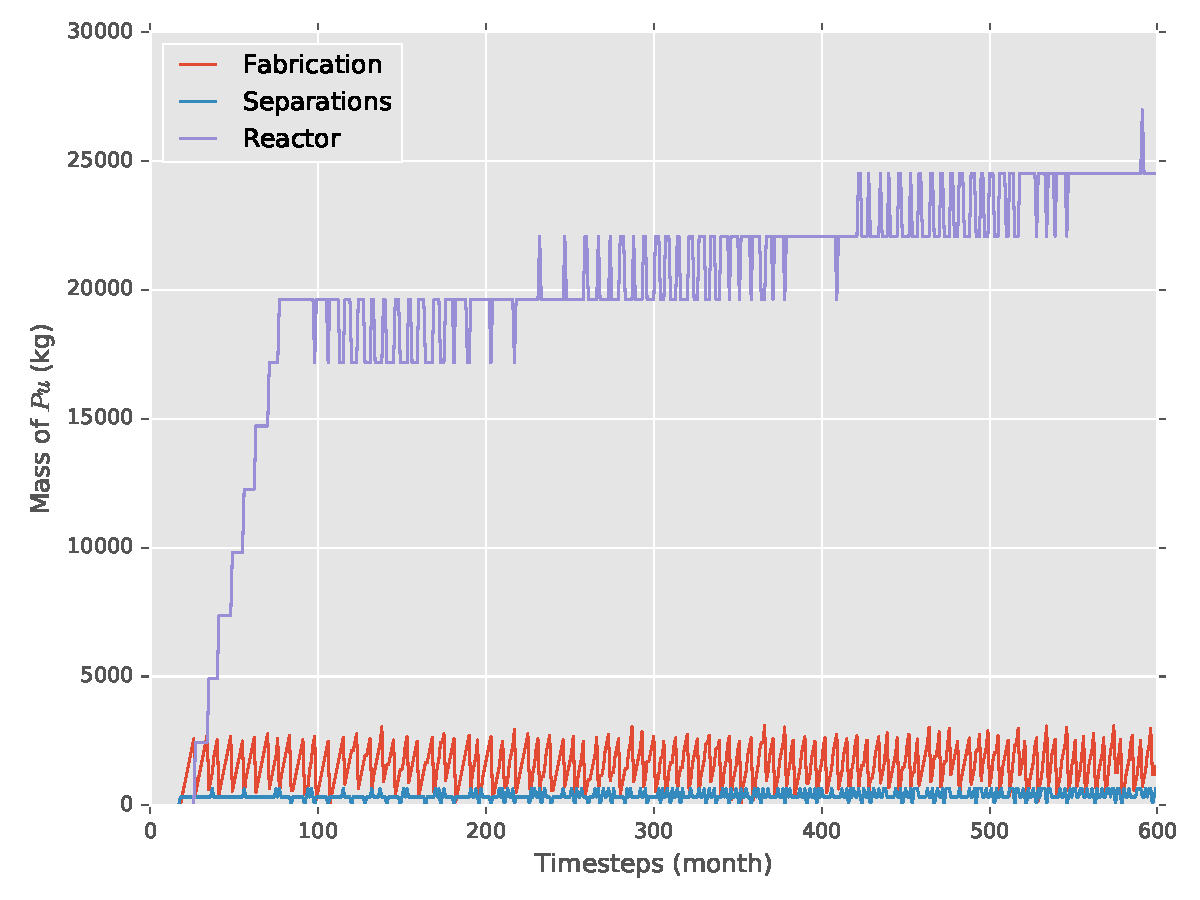
\includegraphics[height=0.3\textheight]{outage_invs_a.pdf}
      \label{fig:baseinv-outage}}
    \vfill 
    \subfloat[Pu inventories in the \outage scenario.]{
      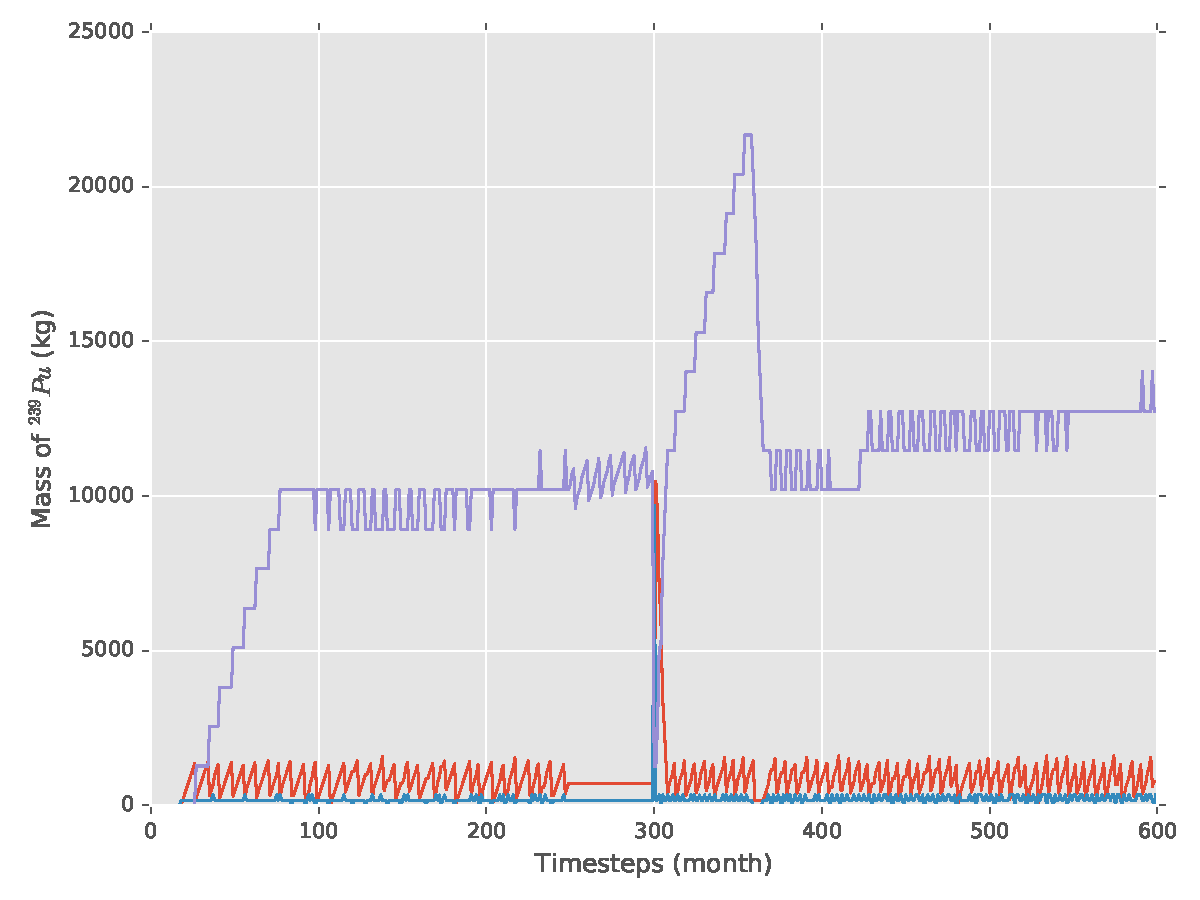
\includegraphics[height=0.3\textheight]{outage_invs_b.pdf}
    \label{fig:outageinv}}
  \end{minipage}%
  \begin{minipage}{0.33\textwidth}
    \centering
    \subfloat[A close-up of the \outage scenario perturbation.]{
      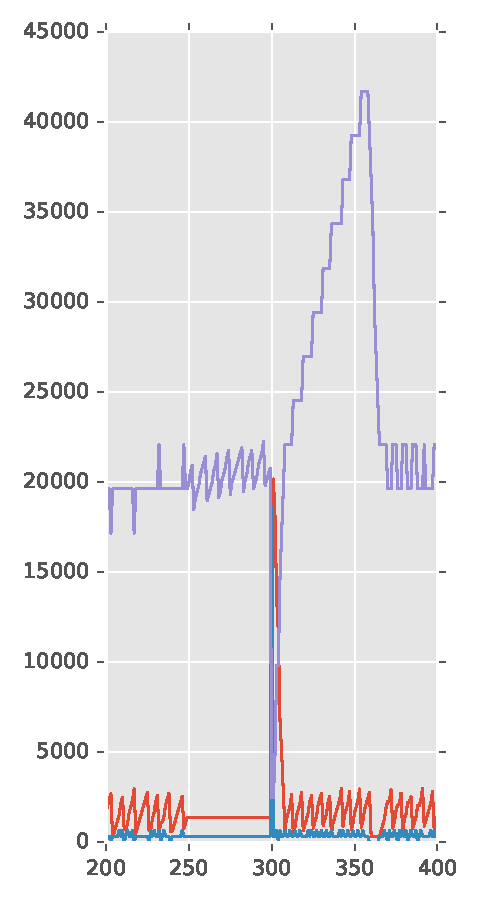
\includegraphics[height=0.6\textheight]{outage_invs_c.pdf}
      \label{fig:outagezoom}}
  \end{minipage}%
  \caption[]{
    \label{fig:outage}
    Facility inventories of Pu in \basecase and \outage scenarios.}
\end{figure}

The dynamic equilibrium behavior changes in the \outage scenario after the
initial outage time, $t_i$, as is observable in Figures \ref{fig:outageinv} and
\ref{fig:outagezoom}. Because the outage occurs in \separations, which takes
input from the \reactors and provides output to \fabrication, the inventories of
both \separations and \fabrication remain constant for the duration of the
outage period. The inventory of Pu in \reactors continues to oscillate
because MOX assemblies are discharged and continue to be sent to \storage,
whereas spent UOX assemblies (with significant Pu inventories) are stored on
site. In the first timestep of renewed service of \separations, $t_f$, the
entirety of the pent-up store of used fuel in \reactors is send to \separations,
reducing the inventory to zero, causing the delta-function behavior in \reactor
flows seen in Figure \ref{fig:outagezoom} at $t = t_f$. \separations then
extracts all of Pu in a single timestep, sending it to \fabrication and
causing the delta-function behavior in \separations flows seen in Figure
\ref{fig:outagezoom} at $t = t_f + 1$. Finally, the stock of Pu in \reactors
after the outage increases due to the higher availability of MOX fuel in
\fabrication, until the dynamic equilibrium returns. The length of the
perturbation is function of both the amount of Pu required per refueling and
the number of refuelings that occurs during the outage. The more refuelings that
happen during the outage, the more excess MOX assemblies can be made, thus
continuing the dynamic equilibrium perturbation.

\subsection{External MOX Supplier: Fuel Cycles with Demand Fungibility}

The DRE allows for both positive and negative perturbations in fuel
availability. While the \outage scenario models a case where there is a
supply-chain disruption, the \external scenario models a case where there is an
injection of a preferred commodity source. An example of such a scenario
occurring in the real world includes the down-blending of military-grade fuel
sources, such as the MOX Fuel Fabrication Facility, in which a preferred fuel
commodity is introduced, and the Megatons to Megawatts (MT2MW) program, where a
preferred fuel fabrication commodity is introduced at the enrichment-fabrication
facility interface.

In the \external scenario, an external source of MOX fuel enters halfway
through the simulation at $t = 250$, creating the fuel cycle shown in Figure
\ref{fig:military_fc}. The total quantity of fuel the external source can provide is
limited to 10 refueling quantities (where reactors refuel one third of their
total core mass in each cycle). Preferences are assigned such that reactors
prefer MOX from its normal cycle over MOX from the external source, i.e.,
$p_{\text{MOX}} > p_{\text{MOX, external}} > p_{\text{UOX}}$. Reactors request each
of the commodities, and thus the first 10 reactors to refuel after the external
source enters the simulation when no original MOX is available will be provided
with MOX from the external facility. Reactors will continue to request fuel from the
external facility for the remainder of the simulation, but will not receive any due
to the limited total inventory. This injection of a new fuel source also serves to
perturb the supply chain by delaying the amount of spent UOX available for
recycling.

\begin{figure}
  \begin{center}
    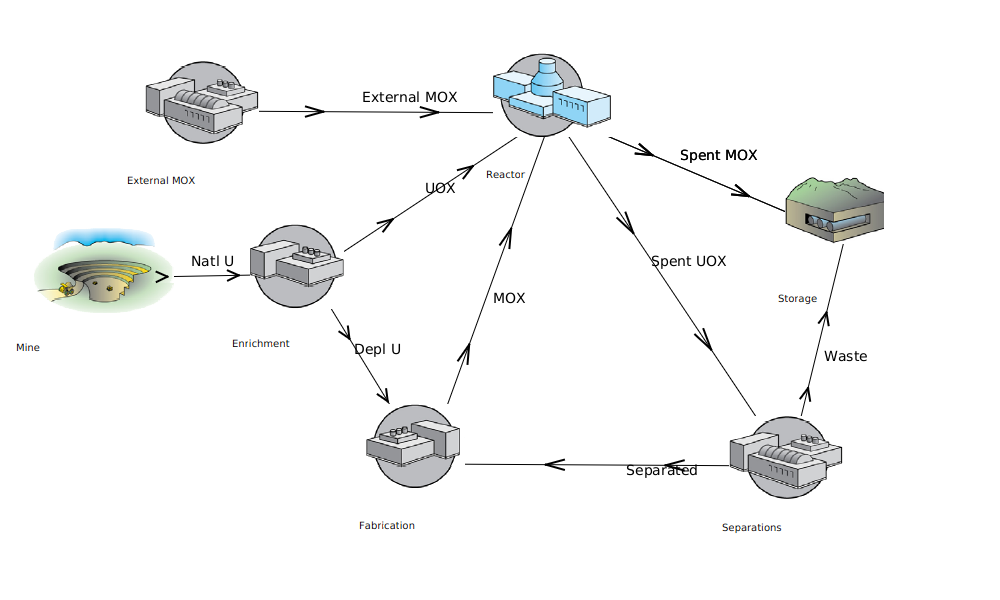
\includegraphics[width=\columnwidth]{external_fc}
    \caption[]{
      \label{fig:military_fc}
      Material routing between in the \external scenario fuel
      cycle. Possible arc flows are labeled with commodity names.}
  \end{center}
\end{figure}

The dynamic equilibrium of Pu inventories again changes with the \external
perturbation, as shown in Figure \ref{fig:military}. A number of new features
arise, however. First, the equilibrium value during the initial transient
increases by the total quantity of refueling quantities available from the
external source of MOX (in this case 10 refueling quantities). Second, the
equilibrium value upon exiting the transient is lower than the value upon its
entrance. This is due to the fact that the amount of spent UOX in the overall
recycle system has decreased, due to the usage of external MOX, thus reducing
the availability of MOX. The system has been shocked into a new dynamic
equilibrium, with Pu values slightly lower than the previous
equilibrium. This suggests that the injection of external recycled fuel can
reduce the level of which a system can sustain a recycling fuel cycle. Finally,
a small lag can be seen in the inventory of Pu in \fabrication, which is due
to a loss of available spent UOX due to the increased presence of spent MOX
exiting reactors that were able to utilize external MOX. The Pu inventories 
recover quickly from this transient, however.

\begin{figure}
  \centering
  \begin{minipage}{0.67\textwidth}
    \centering 
    \subfloat[Pu inventories in the \basecase scenario.]{
      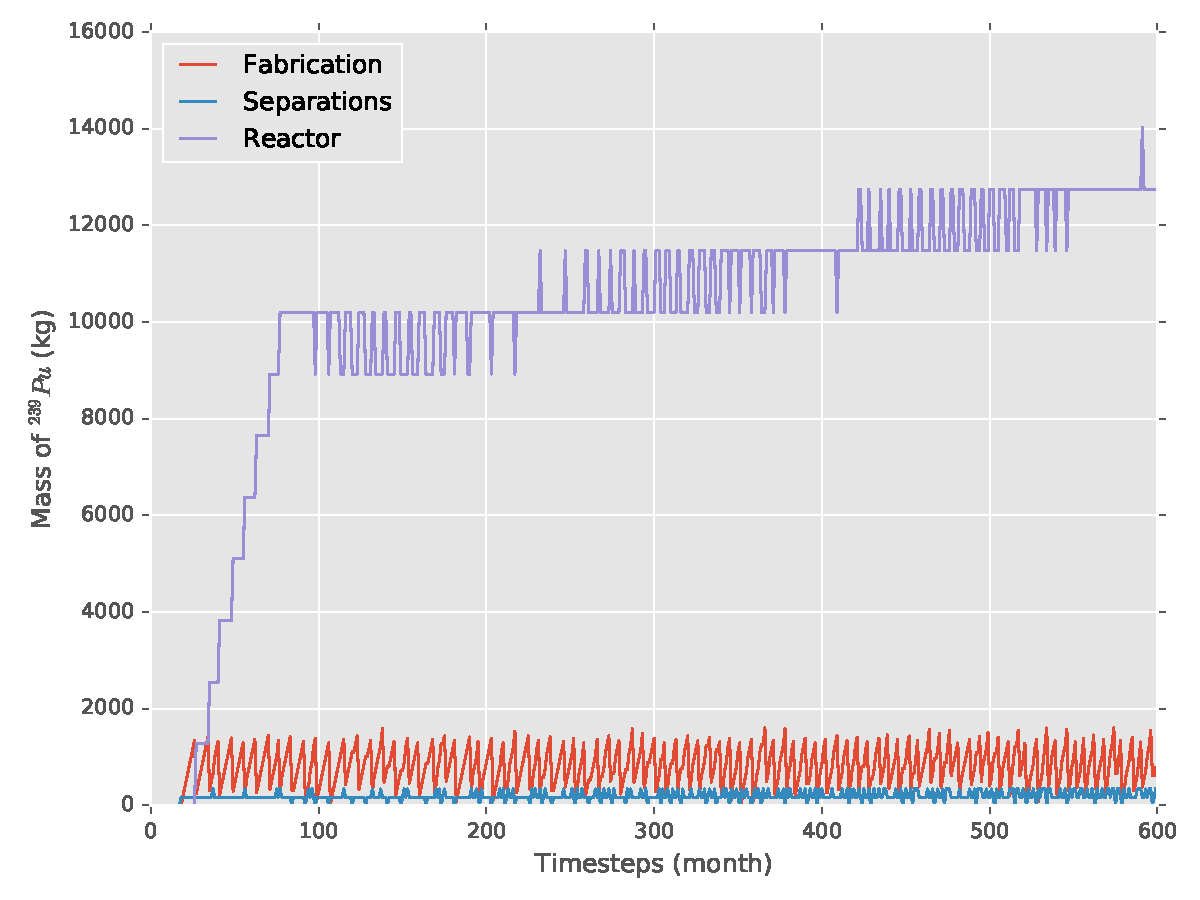
\includegraphics[height=0.3\textheight]{military_invs_a.pdf}
      \label{fig:baseinv-military}}
    \vfill 
    \subfloat[Pu inventories in the \external scenario.]{
      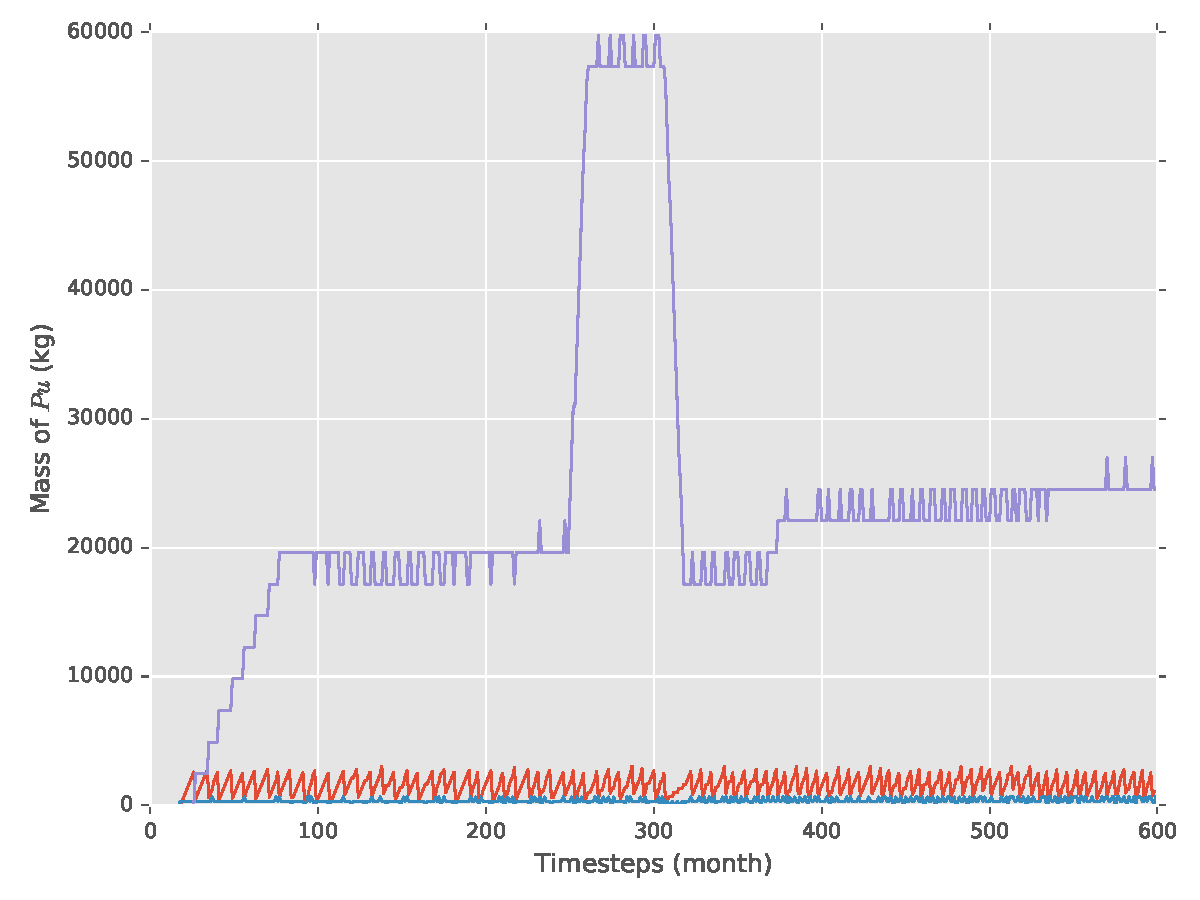
\includegraphics[height=0.3\textheight]{military_invs_b.pdf}
    \label{fig:militaryinv}}
  \end{minipage}%
  \begin{minipage}{0.33\textwidth}
    \centering
    \subfloat[A close-up of the \external scenario perturbation.]{
      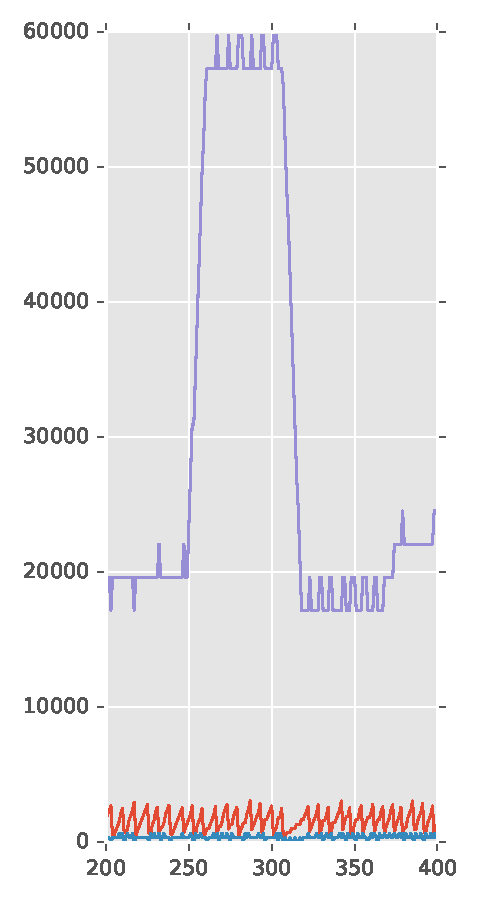
\includegraphics[height=0.6\textheight]{military_invs_c.pdf}
      \label{fig:militaryzoom}}
  \end{minipage}%
  \caption[]{
    \label{fig:military}
    Facility inventories of Pu in \basecase and \external scenarios.}
\end{figure}

\subsection{Regional Tariffs: Fuel Cycles with International Instruments}

One of the novel features of the DRE is the ability for different geographical
and managing entity representations to be laid over otherwise regional-agnostic
fuel cycles and affect the outcome of possible trades between those fuel
cycles. The \tariff two-region scenario showcases the ability to model
such situations.

Two regions, Region A and Region B, are modeled. Region A houses a fuel cycle
with both UOX and MOX-based fuel services, as in the \basecase scenario. The
same total number of \reactors are modeled in the scenario. Region A begins with
15 \reactors and Region B begins with 5 reactors. All reactor deployment as
shown in Figure \ref{fig:deploy} occurs in Region A.

In this scenario, Region A can provide UOX and MOX fuel services to other
regions using a fuel take-back model (all fuel provided as a service is returned
after it has been used in a reactor). Repatriation of fission products to the
lessee region is not modeled in this scenario for purposes of clarity. Region B
contains a simple, once-through fuel cycle. Although the scenario is somewhat
contrived in order to highlight a multi-commodity system under dynamic
behavioral change, such fuel service arrangements are present today in countries
that provide fuel for once-through fuel cycles, e.g., Russia
\cite{wnarussia2016}. The possible flow of commodities between fuel cycles is
shown in Figure \ref{fig:region}.

\begin{figure}
  \begin{center}
    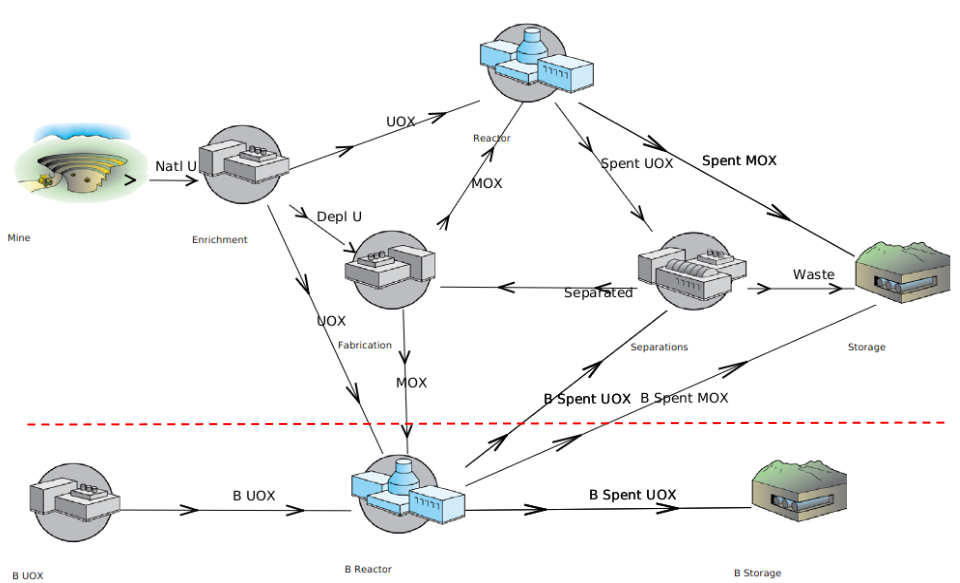
\includegraphics[width=\columnwidth]{tariff_fc_line}
    \caption[]{
      \label{fig:region}
      A two-region set of fuel cycles separated by a dotted-red line. The upper
      region (Region A) includes a one-pass MOX fuel cycle, and the bottom
      region (Region B) includes a once-through fuel cycle connected to the
      one-pass MOX fuel cycle. Note that all spent fuel that originated in
      Region A is returned to Region A's fuel cycle.}
  \end{center}
\end{figure}

Initially, preferences are set such that fuel trade from Region A to
Region B is preferred over Region B's domestic fuel production. In other words, a
preference distribution for fuel supplied to Region B has the following
relation

\begin{equation}\label{eqn:bigdefault}
  p_{MOX, a} > p_{UOX, a} > p_{UOX, b} > 1.
\end{equation}

\noindent
This preference distribution implies that Region B's domestic fuel cycle will
never be utilized -- it will always be fueled by Region A, as long as Region A
has available capacity. 

At some time $t_0$, a time-varying tariff is applied by Region B which perturbs
preference values along arcs connecting Region A fuel suppliers with Region B
fuel consumers. Consider a tariff defined by function in Equation
\ref{eqn:tariff} with preferences adhering to the relation provided in Equation
\ref{eqn:bigp1}, which guarantees a strict preference ordering under $f(t)$.

\begin{equation}\label{eqn:tariff}
f(t)
\begin{cases}
1, & \text{if } t < t_0 \\
\frac{p_{UOX, b} - 1}{p_{UOX, a}}, & \text{if } t_0 \leq t < t_1 \\
\frac{p_{UOX, b} - 1}{p_{MOX, a}}, & \text{if } t_1 \leq t < t_2
\end{cases} 
\end{equation}

\begin{equation}\label{eqn:bigp1}
  p_{UOX, b} \left( 1 - \frac{p_{UOX, a}}{p_{MOX, a}} \right) > 1.
\end{equation}

Choosing nominal values that satisfy Equations \ref{eqn:bigdefault} and
\ref{eqn:bigp1}, e.g., $p_{MOX, a} = 9$, $p_{UOX, a} = 4$, and $p_{UOX, b} = 2$,
one arrives at actual preference values as shown in Figure \ref{fig:prefs}. In
the \tariff scenario, $t_0$ is chosen to be 150 and $t_1$ is set to 300. The DRE
naturally handles the flow of commodities between \texttt{Facility} agents in
each \texttt{Region}, allowing the application of tariffs by the \texttt{Region}
agents.

\begin{figure}
  \begin{center}
    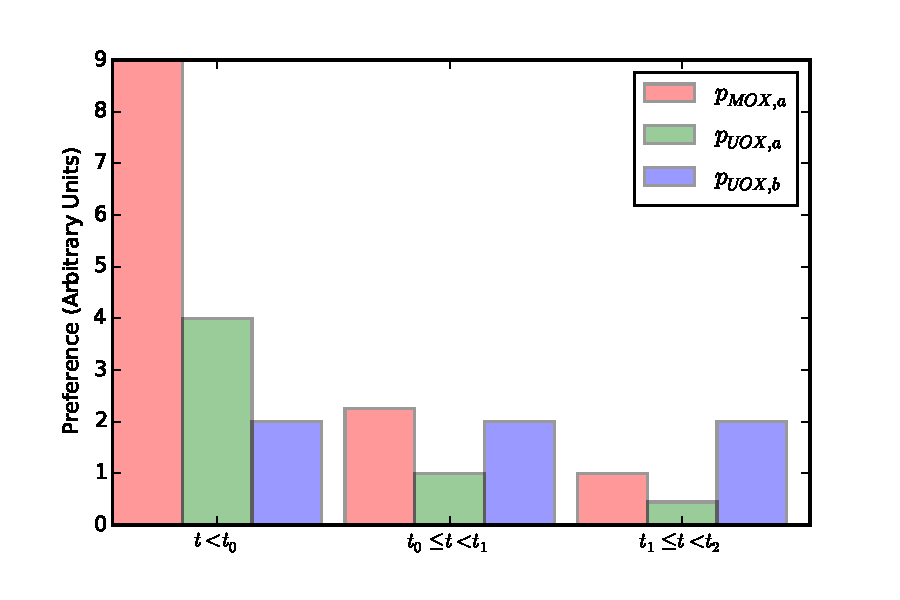
\includegraphics[width=\columnwidth]{tariff_prefs.pdf}
    \caption[]{
      \label{fig:prefs}
      Preference values for reactors in Region B for available fuel commodities
      in Region B as a function of time.}
  \end{center}
\end{figure}

The effects of time-dependent tariff application on the simulation can be seen
in Figure \ref{fig:tariff}. The front-end of Region B's fuel cycle is not
utilized until $t > t_0$; all fuel is provided from Region A. After $t_0$, the
majority of the fuel services required by \reactors in Region B comes from
Region B's own front end. However, it is still able to utilize the MOX-based
fuel services from Region A. Finally, after the final tariff is applied at
$t_1$, Region B's \reactors stop utilizing Region A's fuel cycle entirely.    

\begin{figure}
  \begin{center}
    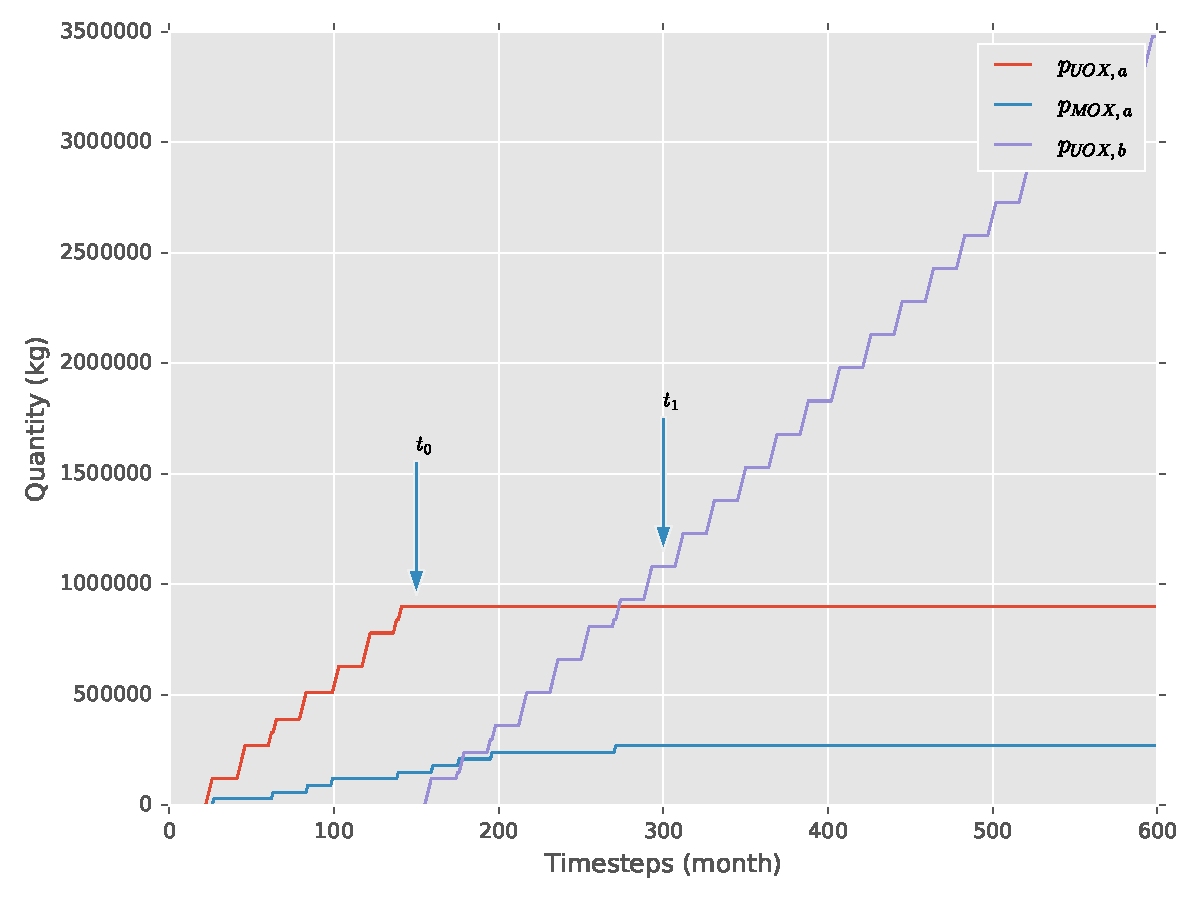
\includegraphics[width=\columnwidth]{tariff_b_reactor_flow.pdf}
    \caption[]{
      \label{fig:tariff}
      Cumulative flow of fuel into \reactors in Region B.}
  \end{center}
\end{figure}

\subsection{Comparisons between Scenarios}

In each scenario, the total amount of electricity generated is identical in
order to compare the mechanics and results of fuel supply and demand. Therefore,
comparisons between all scenarios is most easily made by observing the total
fuel usage by reactors for each commodity type. A summary of this metric is
provided in Figure \ref{fig:flows}. Figure \ref{fig:uoxflow} displays the
cumulative flow of UOX fuel into reactors over all scenarios which shows a
number of interesting effects. First, the \external scenario has the lowest
cumulative flow, which is expected of a scenario in which an external source of
non-UOX is provided.  The \outage scenario initially deviates from the \basecase
scenario, but eventually returns to match its cumulative UOX usage. This is due
to the fact that in the defined system, outages simply serve to store fuel. When
sufficient time has past after the outage, the system returns to its dynamic
equilibrium. Finally, the \tariff scenario utilizes the most UOX fuel of all,
providing an interesting case study of the effects of dynamic equilibrium. In
the \tariff scenario, there is a population of reactors that prefers UOX fuel
that is not sent to \separations (i.e., the UOX fuel in its own Region) over all
other sources in the simulation. Therefore, the population of Pu is reduced,
which reduces both the quantity and frequency of MOX availability. This, in
turn, increases overall UOX consumption. In short, MOX availability decreases
due to upstream supply chain effects, causing an increase in overall UOX
consumption.

Figure \ref{fig:moxflow} showcases the cumulative flow of MOX fuel into all
reactors as a function of simulation time step. Because reactors can be fueled
only with UOX or MOX, it represents the inverse of Figure \ref{fig:uoxflow}. For
example, whereas the \tariff scenario utilizes the most UOX, it utilizes the
least MOX for the same reasons. A number of additional features can be observed
in Figure \ref{fig:moxflow} dealing with departures from dynamic equilibrium of
the \basecase scenario. The undershooting and then overshooting of MOX
consumption in the \outage scenario is visible. During the outage, less MOX is
consumed, but immediately after the outage, excess MOX is consumed until there
is a return to dynamic equilibrium. Additionally, a reduction in the total
amount of MOX (sourced from recycled UOX) consumed is observed in the \external
scenario. This is due to a reduction in the available recycled UOX supply during
periods of external MOX consumption. In short, for each reload of external MOX,
the system loses a future amount of recyclable UOX.

\begin{figure}
  \centering
  \begin{minipage}{0.9\textwidth}
    \centering
    \subfloat[UOX flow.]{
      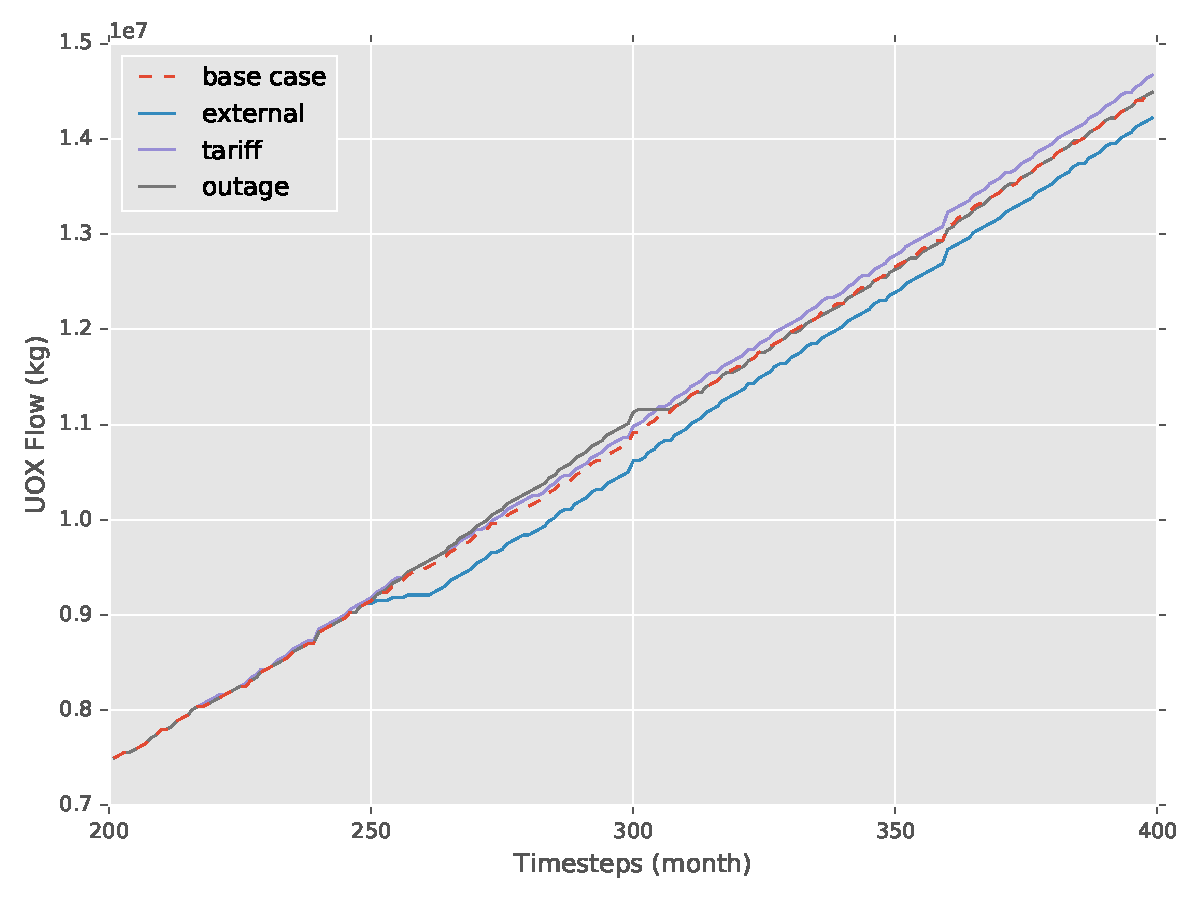
\includegraphics[width=0.9\textwidth]{uox_flow.pdf}\label{fig:uoxflow}}
    \vfill
    \subfloat[MOX flow]{
      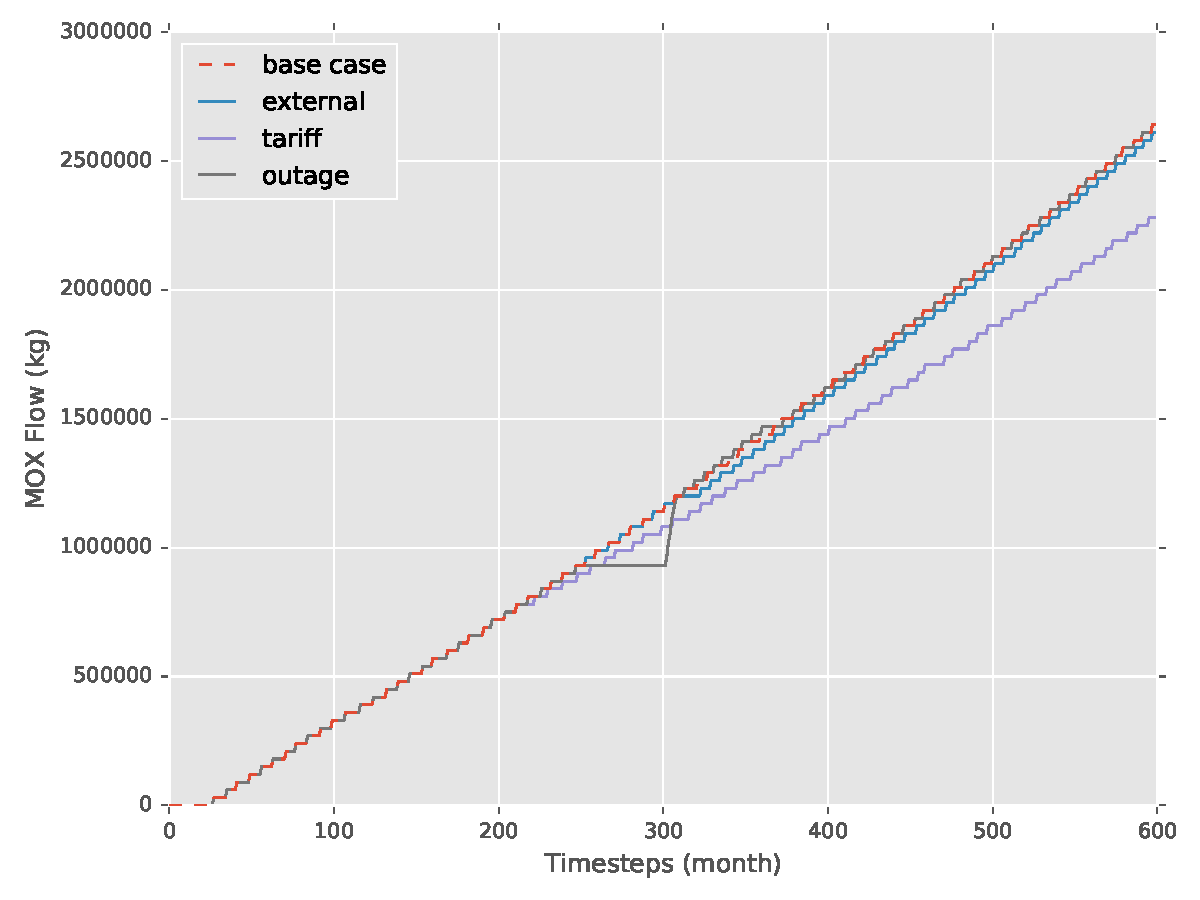
\includegraphics[width=0.9\textwidth]{mox_flow.pdf}\label{fig:moxflow}}
  \end{minipage}%
  \caption[]{
    \label{fig:flows}
    Cumulative flow of fuel in all Scenarios. The timestep period between 200
    and 400 is chosen to highlight all relevant transients. }
\end{figure}

\subsection{Solver Comparisons}

Each of the above scenarios was executed by solving the DRE using both the
\greedy heuristic and full optimization (results are shown from the \greedy
heuristic cases for clarity). Differences in simulation time are observed, as
shown in Table \ref{tbl:timing}. Solving the DRE with full optimization takes
approximately twice as long as solving it with the \greedy heuristic in these
simulations. These are small simulations and one can expect this solution time
gap to increase exponentially with simulation size, as solutions to MILPs
increase exponentially with time and the \greedy heuristic is a polynomial-time
algorithm. The primary component of simulation size that is of concern to
solution time is the total number of supply and request nodes in each
problem. These will increase with the number of entities in the simulation, the
number of commodities, and the connectedness of entities (i.e., the number of
potential transfers between entities).

\begin{table}[]
\centering
\caption{Solution times required for full simulation runs of each solver type in
  each scenario. Simulations were performed on a Macbook Air with a duel-core i5
  2.6 GHz processor using a Ubuntu 14.04 operating system.}
\label{tbl:timing}
\begin{tabular}{llr}
\toprule
Scenario & Solver & Time (s)           \\
\midrule
\basecase & cbc &     6.306 \\
          & greedy &     4.169 \\
\external & cbc &     6.371 \\
          & greedy &     3.149 \\
\outage & cbc &     5.978 \\
          & greedy &     3.161 \\
\tariff & cbc &     6.074 \\
          & greedy &     3.079 \\
\bottomrule
\end{tabular}
\end{table}

Each of the results in Table \ref{tbl:timing} is with respect to the simple
scenarios presented in this paper. In order to ascertain a sense of how each
solver will work with larger scenarios, the \basecase scenario was run an
additional time after modifying the reactor deployment schedule as follows: in
each instance when a single reactor would be deployed, five reactors are
deployed instead, increasing the total reactor population by a factor for five
to approximately 150. The greedy and cbc \basecase scenarios solved in 10.7 and
20.8 seconds, respectively. This implies that there is not a clear linear
relationship between solution time of a full simulation run and the number of
entities in the simulation for either solver -- there are likely additional
simulation dynamics occurring outside of the DRE that affect solution
times. Additionally, this simple exercise shows that simulations of reactor
populations approximately the size of the United States reactor fleet can be
solved in very reasonable times.

Interestingly, slight differences in simulation results was also observed
between the two solvers. This is due to time-steps in which there is problem
degeneracy, i.e., where multiple optimal solutions exist. Consider a timestep,
$t_i$, in which one reactor is refueling and another reactor is entering the
simulation. Four total quantities of fuel are requested - one refueling batch
and three initial core batches. Consider further that one batch of MOX fuel is
available. Because reactors all make requests to the DRE with identical
preferences, there are four degenerate optimal solutions -- one for each
potential assignment of the MOX batch. This leads to three potential simulation
futures, one in which the MOX batch is ejected after one cycle (if it assigned
to the refueling reactor or to the initial spot of the new reactor), one in
which the MOX batch is ejected after two cycles, and a third after three
cycles. In each simulation future, the quantity of fuel in the recycle loop at
$t > t_i$ is different, causing differing future behavior and overall simulation
results.

\section{Conclusions}


%Don't forget there is text in \texttt{old.tex}.
%\section{\textbf{Previous Text, Use What is Needed}}

%%%%%
% Old Motivation Section
%%%%%

Fuel cycle simulation involves a number of components: modeling in-facility
processes (e.g. fuel transmutation), determining facility deployment, and
determining the flow of resources between facilities. Because Cyclus uses an
agent-based modeling approach, each component can be addressed
individually. Facility agents house in-facility process logic. Region or
Institution agents are contain the facility deployment logic. The Cyclus kernel,
informed by agents in a simulation, manages the determination of resource flow
via a multi-commodity material routing model, informed by the rich literature of
supply-chain modeling and optimization.

\subsection{The Material Routing Problem}

The multicommodity supply chain model is a well studied problem. Its goal is to
determine the flow of commodities between suppliers, consumers, and, optionally,
storage locations. A preliminary formulation has been previously explored
\cite{gidden_agent-based_2013}. When applied to the nuclear fuel cycle, this
work terms the resulting problem formulation the Material Routing Problem (MRP).

\subsubsection{Fuel Cycle Models}

Prior work in the fuel cycle simulation field has treated the problem lightly if
at all. Many simulators have simple determination logic built in to their
model. For example, system dynamics approaches generally assign each commodity a
stock and flow, and flow determination logic, if any, is translated into
cofficients of the system dynamics equations. Importantly, adding a new
commodity involves changing the underlying model, which can be a time consuming
task \cite{guerin_impact_2009}.

\subsubsection{Supply-Demand Models}

Modeling supply and demand in a supply-chain context is a field with a rich body
of literature.

Agent-based modeling approaches have also been implemented \cite{julka_agent-based_2002}.

\subsection{Fuel Cycle Concerns}

The nuclear fuel cycle has a number of concerns that must be met by a
multicommodity supply-demand formulation.

\subsubsection{Physics}

A formulation must allow for constraints based on the physics of in-facility processes. 

% eg custom constraints

\subsubsection{Fuel Forms}

A formulation must allow for the variety of forms material can take within the
nuclear fuel cycle. Specifically, any formulation must allow for quantized
material transfers, representing fuel assemblies.

% eg assemblies

\subsubsection{Institutions and Regions}

A formulation must allow for institutional and regional effects to affect the flow of resources.

% eg preferences

\subsection{Cyclus Concerns}

Cyclus must provide an abstraction that translates the supply and demand of
resource objects, e.g. \textit{Material}, from an agent context to an instance
of the MRP. 

% general API and extendable formulation


%%%%%
% Old Methods Section
%%%%%

\subsection{Modeling Supply \& Demand}

\subsubsection{Agent Communication}

An agent communication interface is used to determine supply and demand. The
communication execution is implemented in phases. First, a request for bids
(RFB) phase is executed to determine demand. Next, and response to request for
bids (RRFB) phase is executed to determine supply.

% RFB, RRFB phases

\subsubsection{Graph Representation}

Supply and demand is then translated into an \textit{ExchangeGraph}, stripping
away any derived \textit{Resource} object specialization. 

% mention separability into req/sup cases

\subsubsection{Mixed Integer-Linear Problem Representation}

In order to solve the MRP with mathematical programming solvers, a separate
translation protocol was implemented to translate instances of an
\textit{ExchangeGraph} into an instance of a mixed integer-linear (MILP) problem
using the standardized Open Solver Interface (OSI). %cite osi

\subsection{Solvers}

\subsubsection{A Greedy Heuristic}

A custom heuristic was implemented that utilizes domain-level knowledge of the
resource exchange interface in Cyclus.

\subsubsection{Linear Programming}

In the case in which partial orders are allowed (e.g., when not explicitly
modeling fuel assemblies), the MILP formulation of the MRP simplifies into a
linear program. Linear programs have very fast solution times. This work
utilizes the COIN Linear Program (CLP) solver.

\subsubsection{Mixed-Integer Programming}

% discuss heuristics, cuts, etc.
This work utilizes the COIN Branch and Cut (CBC) solver. 

\subsection{Test Cases}

Solver performance for MILPs is highly dependent on both problem structure and
coefficient values of a given instance. In the absence of a large number of
instances mined from user-run simulations, test cases must be generated. These
cases are designed to explore the behavior of the model as simulation entity
behavior becomes more precise (e.g., modeling individual assemblies) and the
number of simulation entities grows.

\subsubsection{Reactor Request Case}

A description of the RR case.

\subsubsection{Reactor Supply Case}

A description of the RS case.

\subsection{Analysis Platform}

A discussion of Cyclopts, highlighting notion of parameter space, conversion
from parameters to instances, execution, output, and analysis. 

\subsubsection{High Throughput Computing Execution}

Discuss interaction with condor, highlighting specialized nodes used for timing study.


%%%%%%%%%%%%%%%%%%%%%%%%%%%%%%%%%%%%%%%%%%%%%%%%%%%%%%%%%%%%%%%%%%%%%%%%%%%%%%%%
\section*{Acknowledgements}

The authors would like to thank the Nuclear Engineering University Program
(NEUP) for their generous support in the form of both an Integrated University
Program (IUP) fellowship as well as the grants DOE-NE00120341 and
DOE-NE0000673. The authors would also like to thank all developers of the
\Cyclus simulator, especially Kyle Oliver, Dr. Kathryn Huff, Dr. Anthony
Scopatz, Dr. Robert Carlsen, and Arrielle Opotowsky. Finally, the authors would
also like to thank Drs. James Luedtke, Michael Corradini, Laura McLay, and Erich
Schneider for their comments on the development of the methodology of the paper.

\newpage
\section*{\refname}
\bibliography{refs}
\end{document}
